%\renewcommand{\tabularxcolumn}[1]{m{#1}}
%\newcolumntype{Y}{>{\centering\arraybackslash}X}
%\newcolumntype{R}{>{\flushright\arraybackslash}X}



\renewcommand{\thesection}{\arabic{chapter}.\arabic{section}}



\chapter{Dynamics of the Electricity Day-Ahead Market : Supply Function Equilibria and Ramping Costs}
\label{chap:ch1}
\cleardoublepage

\doublespacing
\section{Introduction}
In this chapter, we introduce ramping costs to the theoretical framework of supply function equilibria. \\

Supply function equilibria are used as a theoretical approach to describe the electricity market on which suppliers bid actual functions contrary to most markets, where one's assumptions about demand and supply curves never translate to agents actually bidding on these objects. The most striking results of this litterature are that there exists many (in fact a continuum) of Nash equilibria, that all of those equilibria are ex-post optimal, and that they exhibit always positive prices. \\

The ex-post optimality implies that once an equilibrium is reached, this equilibrium shouldn't change from auction to auction, given that the cost structure remains constant, even when new information is gathered. However, the observation of the hourly bids on the day-ahead electricity market shows that bids indeed do change from hour to hour. There are many reasons for which the bids might change from one another. \\

The first is that power plants are brought online or offline to face varying levels of demand for electricity. In so doing, the cost structure of the suppliers changes, which can justify changes in bids. The second is that changes in production are costly in and of themselves, that is, there exists ramping costs associated to the production of electricity. This effect, although technically well supported, also sees support from the existence of negative prices from time to time on the electricity market, on days of high production and low demand. These cases show that subsidizing consumption is less costly than not producing for suppliers. \\

In this chapter, we propose a theoretical framework to account for these ramping costs.\\

We choose to model the discrete time bidding as a continuous time process.  This allows us to bring to the litterature about supply function equilibria powerful mathematical tools mostly used in option pricing, that is stochastic dynamics: we want to model ramping costs, i.e. costs associated to the variation in production, while retaining the key ingredient brought by \cite{KM}, i.e. the uncertainty, through the use of brownians, and more precisely, It\={o} processes. These tools are the same introduced in the recent litterature on dynamic games, see for example \cite{sannikov2016dynamic}. However, where the focus of this litterature is to revisit classical results of repeated games in the context of a time-continuous framework as well as to describe real world cases more appropriately captured by continuous time models (for example trading), our focus is to be able to capture the effects of ramping costs on the electricity day-ahead market, a market which is discrete in nature.\\

We obtain a rich and tractable model that yields results that contrast strongly with past results from the litterature. First, in the specific case of linear demand and linear costs we obtain a unique Nash equilibria, which contrasts with the usual continuum of Nash equilibria in the supply function equilibria litterature. Second, our solutions are not ex-post optimal, meaning that gathering information about the expected future evolution of demand yields different optimal strategies for suppliers, which in turn means that producers in our framework have a motive for submitting different supply functions from one time step to the next. Third, we have closed form solutions which yield specific predictions about the evolution of bids under uncertainty, namely that when uncertainty increase, suppliers submit steeper supply schedules in order to transmit more of these shocks to changes in price and not quantities, which are costly due to the existence of ramping costs. Finally, and less importantly, our framework justifies the existence of negative prices \footnote{Note that such negative prices happen, a few hours a year for example in France or Germany, for example in 2017 there were 146 such hours on 24 days in Germany \cite{epexnegP}} by producers being willing to pay consumers to consume more in order to avoid facing large variations in production, in contrast to everywhere positive schedules in the case of the supply function equilibria litterature.\\

\subsection{Litterature review}
The electricity markets have flourished in Europe during the 1990s during the wave of privatization. The argument for their creation was one of competition, that was supposed to bring lower prices to the end consumer of electricity.\\

An important specificity to the economics of electricity is that electricity cannot be stored in large amounts, which in turn implies that at every moment production and consumption have to match. This means that in order to have a working electric grid, that is one that can produce electricity at higher levels during the winter and lower levels in summer, one has to have production units ready to be turned on if the demand is high enough, but turned off otherwise. This in turn means that although their existence is required, it is difficult to see how marginal cost pricing can cover their investment costs, which has been a long running argument in the litterature \cite{boiteux1960peak}. For this reason, from the very beginning the issue of the market design was deemed to be crucial to insure that the wished for outcome of the privatization wave came to fruition \cite{green1991reshaping}. \\

Most countries having open the production of electricity to competition have implemented day-ahead markets. As said above, the production and the consumption have to match constantly. The very short term matching is done by automating tiny adjustments around what a producer is already producing in order to match the fluctuating consumption. To plan which plant should be online at which hour of the day however, the day-ahead markets come in. The idea is that producers and big consumers of electricity (either for themselves, or as aggregators of the individual consumptions) are asked to bid demand or supply functions respectively. The market operator then aggregates the demand and supply curves, which yields an equilibrium giving the price and quantities to be produced for each producer.  \\

There has been an active litterature trying to model and measure the market power of oligopolists on these newly created markets \cite{Newgreen, newbery1998competition, green1999electricity}. The models have mainly been based on Klemperer and Meyer 1989's Econometrica founding paper about supply function equilibria \cite{KM} (henceforth known as KM). \\

This paper builds upon previous results about competition in supply schedules without uncertainty \cite{grossman1981nash}, which yielded a very high multiplicity of equilibria. KM add a key ingredient: uncertainty about the demand schedule facing the suppliers. This addition reduces greatly the multiplicity, and adds more structure to it, although in this framework there is still a continuum of Nash equilibria, which are always pinned between Cournot and Bertrand outcomes. \\

Groundbreaking and fertile, the original model by KM studied how demand uncertainty collapses dramatically the set of available supply function equilibria to a well defined continuum when contrasted to the case of competition in supply schedules without uncertainty \cite{grossman1981nash}. These equilibria are always pinned between Cournot and Bertrand outcomes. This continuum collapses further to a single Nash equilibria by considering an infinite support of demand shocks, that is an unbounded distribution of shocks. All of these equilibria are ex-post optimal, meaning that changes in anticipated demand shocks do not impact the actual solutions, but only the parts of the solutions that are actually explored as shocks realize, a very strong result. \\

The electricity markets litterature has embraced this framework because it is considered to capture some of the structure at play in the electricity markets: the producers do not know what demand they are going to face when they choose their supply schedule, the demand side is considered much less sophisticated than the supply side, and their demand schedules can therefore be considered to some extent as being exogenous. Some have argued that the schedules submitted in the real markets are discrete and that this discrete nature makes their modelling as continuously differentiable schedules is both incorrect and yields different results from discrete ones \cite{von1993spot}. However recent results suggest that with a sufficient amount of steps both approaches converge \cite{holmberg2008supply}, and indeed we see that recent implementations of the market rules increase the number of steps allowed for a single bid, and consider that these points are linearly joined instead of stepwise.\\

One of the most striking aspects of the supply function equilibria approaches is, as was alluded to above, the multiplicity of Nash equilibria. This result has been generally viewed as the source of the danger of tacit collusion in electricity markets: if there is a continuum of nash equilibria, repeated interactions are feared to be conducive to a convergence of bidding strategies towards the most profitable equilbria \cite{bolle1992supply}. \\

Furthermore, these models abstract away some of the details of the actual markets, reason for which authors which try and evaluate the market power of producers on the electricity markets view their endeavour as painting the situation with an optimistic brush \cite{Newgreen}. \\

Here we will tackle the points raised in the last two paragraphs to some extent. We propose to consider a technical reality of the operating of power plants: their cost structure is history-dependant, more precisely, producing a quantity $q_1$ does not entail the same cost if the previous quantity produced was already $q_1$ or if the previous quantity was different from it. Raising or decreasing production in and of itslef imply costs. By introducing these costs we aim to produce a model capable of capturing more precisely the competition that arises in the electricity markets, and in so doing we will show that the continuum of equilibria caracteristic of supply function equilibria under uncertainty collapses to unique equilibria, which in turn allows us to comment on the question of tacit collusion.\\


%
%One traditional understanding for the role of markets is that a market allows to aggregate information that would be otherwise dispersed. When applying this view to the electricity markets, the litterature has regarded the existence of the capacity market as a way to aggregate information about investment costs when building a plant, the existence of the forward market as a way to aggregate information about the fixed costs, and the existence of the spot market as a way to aggregate information about marginal costs. \\
%
%
%At the same time, the litterature as well as the industry is well aware of the existence of ramping costs, that is costs that depend on the variation of production. We think that the two spot markets can be understood as aggregating information about marginal costs and ramping costs. In this paper we model the day-ahead market using the supply function equilibria framework and considering that there exists ramping costs. This allows us to obtain unique solutions, in contrast to the usual continuum, and to describe the dynamic evolution of the optimal bid in a symmetric oligopoly. It also opens the possibility to distinguish between day-ahead and intraday markets. \\
%
%%However, the spot market is actually divided into two markets: the day-ahead market and the intraday or balancing market, that the litterature does not differentiate clearly.
%
%The supply function equilibria litterature has been active since the seminal paper by Klemperer and Meyer in 1989 \cite{KM} (henceforth known as KM). In the wake of the electricity industry liberalisation, authors, notably Green and Newbery in 1992 \cite{Newgreen}, have used this framework to evaluate the expected level of competition and argue for certain regulatory paths. \\

\subsection{The day-ahead markets}

On the electricity day ahead markets, producers are generally required to submit supply schedules once a day for all the auctions taking place during the next day. The APX (England) and the EPEX (Austria, France, Germany and Switzerland) markets allow hourly auctions \cite{apx,epex}, and EPEX allows for bids comprising up to $256$ price quantity combinations, effectively approximating smooth supply functions. Producers can submit different supply schedules for each individual auction, but every bid must be placed at the same time one day in advance for each block of 24 hours. Customers go through the same process and submit their demand schedules, then the market operator matches supply and demand for each auction. Producers thus have to submit schedules facing uncertain demand, this is the reason for the popularity of supply function equilibria approaches to the electricity market.\\   

However, on this market, bids change from auction to auction. From the point of view of KM's model, this should happen only through a coordination of agents agreeing to collectively swap from one Nash equilibrium to another in the available continuum. Describing these dynamics, however, is increasingly important as the energetic mix is bound to include an increasing fraction of renewables. Power production can be separated in two classes: dispatchable and non-dispatchable technologies. Nuclear, coal, land-fill gas or hydroelectric power generation are mainly dispatchable as one can actually choose their level of production whereas the two rising stars of renewable energy, namely wind and solar, are non-dispatchable: they react to weather conditions. Having these technologies in the mix introduces uncertainty on the production side, which comes down to dispatchable units facing a more uncertain residual demand \cite{Boyle}. In this paper we want to explore how to model these dynamics. \\

Electricity production faces very specific technological constraints. These constraints, generally labelled as ramping costs, vary across production technologies, and have yet to be captured in a model. We propose to do so by introducing a multivariate cost function, depending as always on the quantity produced, but also on the rate at which production varies: $C(S,\frac{dS}{dt})$. We call this class of cost functions dynamic cost functions. We detail which form these costs take, and its shape in section \ref{sec_ramping_costs}.\\

All power plants face maintenance costs. However part of these maintenance costs are induced by the dynamics of production, and can be seen as ramping costs. More precisely, whatever the production technology, fluctuations in production are costly. Indeed, they imply fluctuations in the temperature of the core of the power plant, thus dilation and contraction cycles of the different parts, which cause wear and tear. The industry is aware of these effects \cite{GE}, as well as the litterature, although it focuses mainly on other types of effects, such as the impact on shutdown due to maintenance \cite{rothwell1995dynamic}, some B2B companies even specialize in minimizing the related long term costs. For example, Wartsila Power Plants, a supplier of power plants and tools to forecast long term costs, explains in a white paper \cite{Arima}: 
\begin{quote}
Increased variability in net load demand means that dispatchable generating units have to ramp considerably more steeply and deeper than traditionally, thus increasing wear and tear to components.
\end{quote}
We are going to model these ramping costs through a dynamic cost function, increasing in the absolute value of its second argument: any change in production is costly. This paper will focus on the implications of considering this type of ramping costs. Other types of ramping costs exist, for example startup costs, but they will not be studied in this paper. \\

These effects cannot be captured by traditionnal cost functions depending on the level of production alone. One needs to take into account the actual path leading to a given quantity produced, and more precisely in our only the instantaneous variation, not the whole history. This implies that we need to impose structure on the dynamics of the system while retaining uncertainty, the key ingredient of KM's paper. To do so, we use stochastic dynamics. \\

This seemingly small addition to KM's framework has a lot of implications on the results obtained. The solutions are not ex-post optimal anymore, allowing to account more satisfactorily for the dynamics of optimal supply schedules, and our solutions are unique, even for bounded demand shocks. We also define a novel selection rule to choose from KM's continuum of equilibria. Finally these results open the possibility to distinguish intraday and day-ahead markets. \\ 

%In section \ref{litrev} we will present how this paper contributes to the litterature, i
In section \ref{heur} we will present a heuristic approach to get the intuition of the model. Then, in section \ref{math} we will introduce the mathematical tools needed to use stochastic dynamics in this context, in section \ref{monosolve} and section \ref{oligosolve} we will solve the monopoly and the symmetric oligopoly cases while considering that producers have information about the overall distribution of shocks during the day, but do not have information about differences in the shocks at different dates. Finally in section \ref{dynamics} we will discuss the dynamic variation of the optimal bids, while sections \ref{limits} and \ref{ccl} will respectively cover some limits of this approach and conclude the paper.  

%\section{Litterature Review}\label{litrev}
%TO BE FILLED
\section{Heuristic Description of the Model}\label{heur}
In this section the essence of the model is presented before introducing the proper mathematical tools needed to treat this problem rigorously in the next section. It is thought of as an overview of the mathematical methods that are going to be used, as a way to give a sense of the intent of the modelling choices.\\

As in KM's setup, the aim is to model an oligopoly facing uncertain demand, taken as exogenous. Before the demand shocks are realized, each firm needs to commit on a strategy. Firms also incur costs that not only depend on the level of production but also on the evolution of the production given its anterior level produced. \\

More formally, the producer, as in KM, faces uncertain demand, $D(\theta,p)$, with $\theta$ a stochastic shock to the demand and $p$ the price. We add to that both ramping costs and uncertain dynamics of demand. As we want to keep the key ingredient of KM, the introduction of uncertainty, but take into account the dynamics of this uncertainty, of these demand shocks, we need to add more structure.\\

Consider the following notation, where $\theta(t)$ denotes the value of the stochastic shock at time $t$, whereas $\Theta$ denotes the family of all available time trajectories of our demand shocks. \\

In the real market, bidders submit a finite number of bids once a day, and face the ramping costs inter-period, that is, when production has to be adjusted to reach the subsequent market outcome. The first bit of structure we introduce is that we are going to assume that time is continuous. The second is that ramping costs are incurred continuously, and can be thought of as costs depending on the variation of production over time. Finally we consider that bidders are allowed to submit a different supply schedule for every point in time between $0$ and $T$. This amounts to being asked to submit a surface of strategy in the price-quantity-time space for the next day. \\

The producer maximises her expected profits, and we consider here the simplest case in which the distribution of shocks is static, that is that the distribution of probability of shocks does not depend on time, and the producer is asked by the market operator to submit the same supply schedule for every point in time a day in advance. In an oligopoly, the program maximised by producer $i$ is therefore:

\begin{equation}
\displaystyle{\max_{S_i(p)}}~\mathbb{E}_{\Theta}\left[\int_{0}^{T} \left(p(\theta(t))S_i(p(\theta(t))) -C\left(S_i(p(\theta(t))),\frac{dS_i(p(\theta(t)))}{dt} \right)\right)dt\right]
\end{equation}
with $p(\theta(t))$ the price given the demand shock $\theta(t)$ at date $t$, $S_i(\cdot)$ the supply schedule of producer $i$ and $C(\cdot,\cdot)$ the dynamic cost function. Note that the price depends on $t$ only through $\theta(t)$, i.e. a given level of demand shock implies a given price.  \\

The goal of this section is to provide a first run through of the model, therefore we will not describe here the conditions that must be verified by the different terms of the model. We will simply assume that the dynamic cost function is additively separable between a static and a ramping term, $C(S_i,\frac{dS_i}{dt})=C_s(S_i)+C_r(\frac{dS_i}{dt})$, and that the demand shocks $\theta$ are bounded in $[\underline{\theta},\overline{\theta}]$. Lastly we require the ramping term $C_r(\cdot)=\frac{\gamma}{2}(\cdot)^k$ for clarity, and $k\geq2$ an integer. We distribute the expectation operator and write that $\frac{dS_i}{dt}=\frac{dS_i}{dp}\frac{dp}{d\theta}\frac{d\theta}{dt}=S_i'\cdot \dot{p}\cdot \frac{d\theta}{dt}$, with $X'$ the derivative of univariate function $X$ with respect to its argument, $\dot{X}=\frac{dX}{d\theta}$. \\

With this setup, by distributing the expectation operator over all possible trajectories of shocks, we are able to rewrite the problem without having time $t$ appear explicitly. This point is crucial, as it is what will let us use mathematical tools that will yield our unicity results. The maximization program can indeed be written as follows:
\begin{equation}
\displaystyle{\max_{S_i(p)}}~T\int_{\underline{\theta}}^{\overline{\theta}} f(\theta)\left(p(\theta)S_i(p(\theta)) -C_s(S_i(p(\theta)))-\frac{\gamma}{2}\left(S_i'\cdot\dot{p}\right)^k\mathbb{E}_{\Theta}\left[\left(\frac{d\theta}{dt}\right)^k\middle \vert \theta  \right]\right)d\theta
\label{maxbase}
\end{equation}
with $f(\theta)$ the distribution of shocks, and $\gamma$ the ramping cost parameter capturing the magnitude of the ramping costs. The expected value on the trajectory of shocks of any of the terms above that only depend on $\theta(t)$, that is the value of the shock at a point in time, can be rewritten simply as an integral over the possible values of the shock. \\

We are left with $\mathbb{E}_{\Theta}\left[\left(\frac{d\theta}{dt}\right)^k\middle \vert \theta  \right]$ as the only term that depends on the trajectory of shocks. Take for granted that this term can only depend on $\theta$ for now, this result will be justified properly in the next section. \\

Note now that producer $i$ faces a residual demand so that $S_i(p(\theta(t)))=D(\theta,p(\theta(t)))-S_{-i}(p(\theta(t)))$ which depends only on $\theta$ and $p$, $t$ does not intervene directly, with $S_{-i}$ the aggregate supply schedule of all the other producers, taken as given by producer $i$. This implies that the integrand in eq. \ref{maxbase} depends only on three variables: $\theta$, $p$ and $\dot{p}$.  The maximization program is therefore equivalent to an Euler-Lagrange problem, a very well described mathematical object: $\max_p\int\mathcal{L}(\theta,p,\dot{p})d\theta$.\footnote{The Euler–Lagrange equation is an equation satisfied by a function  $p$ of a real argument $\theta$, which is a stationary point of the functional:

$$ S(q) = \int_a^b \mathcal{L}(\theta,p(\theta),\dot{p}(\theta))dt$$

where:
\begin{enumerate}
\item $p$ is the function to be found:
\begin{align*}
p \colon [a,b] \subset \mathbb{R} &\to X\\
\theta & \mapsto x=p(\theta)
\end{align*}
s.t. $p$ is differentiable
\item $\dot{p}$ is the derivative of $p$ w.r.t. $\theta$:
\begin{align*}
\dot{p} \colon [a,b] &\to T_{p(\theta)}X\\
\theta & \mapsto v=\dot{p}(\theta)
\end{align*}
$T_{p(\theta)}X$ denotes the tangent space to $X$ at the point $p(\theta)$.
\item $\mathcal{L}$ is a real-valued function with continuous first derivatives:
\begin{align*}
\mathcal{L} \colon [a,b] \times TX &\to\mathbb{R}\\
(\theta,x,v) & \mapsto \mathcal{L}(\theta,x,v)
\end{align*}
$T_{p(\theta)}X$ denotes the tangent space to $X$ at the point $p(\theta)$.
\end{enumerate}
}
The information obtained from taking the first-order condition of an Euler-Lagrange problem yields a second order differential equation as well as two boundary conditions: $\frac{\partial\mathcal{L}}{\partial p}=\frac{d}{d\theta}\frac{\partial\mathcal{L}}{\partial \dot{p}}$ and $\frac{\partial\mathcal{L}}{\partial\dot{p}}\big|_{\underline{\theta}}=\frac{\partial\mathcal{L}}{\partial\dot{p}}\big|_{\overline{\theta}}=0$. This is why we obtain unique solutions: if the boundary conditions are not verified there exists profitable deviations. \\

In less mathematical terms, taking ramping costs into account as specified above means that for a given level of shock, the producer not only cares about the optimal level of production for this shock, but also about the optimal slope of the supply schedule at this level of production. Effectively, this means that optimal levels of production cannot be chosen independently for different level of shocks as is the case in KM, thus shrinking the continuum of equilibria. The boundary conditions' argument explains why the continuum not only shrinks, but collapses to a unique equilibrium. \\

Note that if the ramping cost parameter $\gamma$ is taken equal to $0$ we are back to KM's model: one doesn't care about the slope of the supply schedule anymore, and the problem comes down to a pointwise maximization which therefore yields ex-post optimal equilibria. We want to stress that this means that it is not sufficient to specify the dynamics of the shocks to obtain a supply function model that would react to these dynamics, one needs to take into account ramping costs.\\

The maximization program~\ref{maxbase} is a heuristic description of the situation. We want to model the stochastic nature of demand and of its dynamics. We do this by using It\={o} processes, a class of stochastic processes built through brownians, to describe the stochastic trajectory of the demand shocks with respect to time. The difficulty is that brownians are everywhere continuous but nowhere differentiable, therefore the way program~\ref{maxbase} is written, with a term in $\frac{d\theta}{dt}$, is a shortcut.\\

In the next section we introduce the stochastic dynamics properly without using the concept of derivative. 


\section{Stochastic Dynamics}\label{math}

As described in the previous section, we consider that bidders submit surfaces, that is supply schedules for every point in time. The reason to describe a discrete dynamic market as a continuous one is that although discrete time is conceptually more easily understood, continuous time allows to use much more powerful mathematical tools and to obtain closed form solutions, which we think are crucial in gaining intuitive insights about these dynamics. Therefore we consider that demand fluctuates continuously and that ramping costs are incurred instantaneously. This approximation would need to be tested, although it should be noted that day ahead markets operate with hourly or half-hourly periods and producers are therefore facing a reasonable amount of periods each day. \\ 

We want our shock variable to evolve over time in a random fashion. The class of mathematical objects used to describe this are stochastic processes. The simplest stochastic process one can think of, and indeed the most important historically, is a Brownian motion process. \\

Unfortunately, Brownian processes are unbounded, and cannot therefore be used to describe the dynamics of the electricity market in which demand shocks, denoted $\theta(t)$, are bounded: there are no days for which demand is null nor are there days for which demand tends towards infinity. The structure to be imposed on the dynamics of the shocks has to imply bounded shocks.\\

%Our strategy to describe a discrete process as a continuous one is as follows. We know which class of stochastic process we want to use in continuous time that is rich enough to yield interesting dynamics yet still manageable mathematically speaking. We are therefore going to take the discrete approximation of this continuous process, discuss this discrete description, and then decrease its timescale towards $0$ to converge towards the stochastic process. We are first going to describe the target stochastic process that we will be using throughout this paper, before illustrating how we go from a discrete description to a continuous one. \\
%
%In the electricity market, demand shocks, denoted $\theta(t)$, are bounded: there are no days for which demand is null nor are there days for which demand tends towards infinity. The structure to be imposed on the dynamics of the shocks has to imply bounded shocks. \\

\subsection{The stochastic process}
A regular candidate for richer stochastic dynamics than a simple brownian process is an Ornstein–Uhlenbeck process. Unfortunately for us, such a process has unbounded support. We are going to use a richer set of stochastic processes: It\={o} processes. \\

The simplest It\={o} process one can consider that leads to bounded shocks is defined by the following stochastic differential equation (SDE) \cite{enveloppe}:
\begin{equation}
d\theta(t)=-2\theta(t) dt+\sqrt{1-\theta(t)^2}dB_t
\label{eqSDE}
\end{equation}
with $B_t$ a brownian and $dX$ an infinitesimal variation of quantity $X$. Its extended version will happen to be very useful in the rest of this chapter, as it leads to a quadratic distribution of shocks, a property that will allow us to obtain closed form solutions.\\

Observe that this SDE is formed by a deterministic mean-returning term $-2\theta(t) dt$ and a bounded stochastic one $\sqrt{1-\theta(t)^2}dB_t$. As $\theta(t)$ approaches $-1$ or $1$ the stochastic term goes to $0$, thus $\theta(t)\in [-1,1]$.  Without loss of generality we can restrain ourselves to this special case. Other bounded supports, $\theta\in[\underline{\theta},\overline{\theta}]$, can be captured through renormalizations of $\theta$. \\

Such a stochastic process has a distribution of probability $f(\theta)$ given by Fokker-Planck's equation, easily solved here. In the general case of an It\={o} process given by SDE \ref{sdegen}, one obtains in \ref{FokP} the generic Fokker-Planck equation for its distribution of probability $f(\theta,t)$. This equation allows, given an initial condition on the distribution of probability of the variable, to observe how this distribution evolves to reach the steady state distribution, that is the limit distribution that any initial condition yields. If one knows the value of the stochastic variable at one point in time, one can use this equation to obtain the spread in its distribution over time. 
\begin{flalign}
&d\theta=\mu(\theta,t)dt+\sigma(\theta,t)dB_t&\label{sdegen}\\ 
&\frac{\partial}{\partial t}f(\theta,t)=\frac{\partial}{\partial \theta}(\mu(\theta,t)f(\theta,t))+\frac{1}{2}\frac{\partial^2}{\partial \theta^2}(\sigma(\theta,t)^2f(\theta,t))&\label{FokP}
\end{flalign}

Here, for SDE \ref{eqSDE}, this yields that $f(\theta)=\frac{3}{4}(1-\theta^2)$ on $[-1,1]$ and $0$ elsewhere.\\

\subsection{The ramping costs}
\label{sec_ramping_costs}
In the rest of the paper we are going to consider quadratic ramping costs. More precisely we consider the costs induced by fluctuations in the production level. As described in the introduction, fluctuations imply increased wear and tear, whether the production is increasing or decreasing. In addition, these ramping costs are null in the absence of fluctuations. This means that they can be captured by a function $C_r(\cdot)$ verifying $C_r(0)=0$, $C_r(\cdot)\geq0$ and increasing in the absolute value of its argument. In the absence of more detailed knowledge about the actual shape of these ramping costs, it seems reasonable to consider a quadratic cost function, that is the first term in a Taylor expansion of the actual real ramping cost function. \\

We cannot compute $\frac{d\theta}{dt}$ as it appears in Eq.~\ref{maxbase}, as a stochastic process, although everywhere continuous, is nowhere differentiable. The goal of this section is to express properly the maximization program of the producer that we presented rapidly in Eq.~\ref{maxbase}, and most importantly, to introduce properly how we can work in continuous time with a cost function which depends on fluctuations, and fluctuations which are nowhere differentiable.\\

We are therefore going to first consider the discrete case of a random walk of timestep $\Delta t$ which converges towards the It\={o} process \ref{sdegen}, using the Euler-Maruyama approximation \cite{kloeden2011numerical}\footnote{This formula can be found on page 305. This book focuses on numerical approximations of continuous stochastic processes, which is the reverse of what we are doing here, but it is only in such numeric-centric books that this scheme is introduced. For a more general approach to stochastic differentiel equations, see \cite{oksendal2003stochastic}}, a generalization of the Euler method to stochastic differential equations. We consider a Markov chain $Y$ defined as follows: 

\begin{equation}
\Delta Y_n=Y_{n+1}-Y_n= \mu(Y_n,n \Delta t)\Delta t+\sigma (Y_n,n \Delta t)\Delta B_n
\end{equation}
where $\Delta B_n=B_{(n+1)\Delta t}-B_{n\Delta t}$. These $\Delta B_n$ are \emph{i.i.d.} normal random variables of mean $0$ and variance $\Delta t$. Note that as $\Delta t$ is taken towards $0$, this Markov chain converges towards its underlying stochastic process defined by eq.(\ref{sdegen}).\\

The ramping costs are taken as quadratic in the variation of the production, and also depend on a ramping cost parameter $\Gamma(\Delta t)$, that is the cost per unit of quadratic variation at horizon $\Delta t$, so we compute the following quantity: 

\begin{equation}
\mathbb{E}\left[\frac{\Gamma(\Delta t)}{2}\cdot\left(\frac{Y_{n+1}-Y_n}{\Delta t}\right)^2\middle \vert Y_n  \right]=\frac{\Gamma(\Delta t)}{2}\cdot\frac{\sigma (Y_n,n \Delta t)^2}{\Delta t}
\label{markovariation}
\end{equation}

For this quantity to converge to a finite value when the Markov chain is taken towards its underlying stochastic process we have to consider that for small enough timescales, the ramping cost parameter $\Gamma(\Delta t)$ is linear in $\Delta t$, i.e. $\Gamma(\Delta t)=\gamma \Delta t +o(\Delta t)$. Mathematically, if $\Gamma(\Delta t)$ had a slower than linear relationship at small timescales, the ramping costs would diverge, and if it was faster they would converge to $0$. A physical constraint, namely thermal inertia, ensures that the ramping cost parameter does actually behave in this way.\footnote{Ramping costs come from thermal fluctuations in the core of the plant. Therefore we have to describe how temperature responds to fluctuations in production. Thermal inertia acts as a low pass filter, meaning that it smoothes out fluctuations on short timescales. Think about heating a saucepan full of water: although lighting the stove is almost instantaneous, the temperature of the water being heated increases only progressively, in an exponential fashion that is therefore linear in time for short timescales. } \\

%For more details about this, see appendix \ref{rampingcostsappendix}.\\

Consider for now that the mean function $\mu$ and the variance function $\sigma$ from eq. \ref{sdegen} do not depend on time explicitly and are therefore written $\mu(\theta)$ and $\sigma(\theta)$. Consider now a transformation $T(\cdot)$ that we apply to the Markov chain $Y$. Then:
\begin{equation}
\mathbb{E}\left[\frac{\Gamma(\Delta t)}{2}\cdot\left(\frac{T(Y_{n+1})-T(Y_n)}{\Delta t}\right)^2\middle \vert Y_n  \right]= \mathbb{E}\left[\frac{\Gamma(\Delta t)}{2}\cdot\left(\frac{T(Y_{n+1})-T(Y_n)}{Y_{n+1}-Y_n}\cdot\frac{Y_{n+1}-Y_n}{\Delta t}\right)^2\middle \vert Y_n  \right]    
\label{markovcomposed}
\end{equation}

And in the limit where the markov process $Y$ converges towards the It\={o} process $\theta$ of equation \ref{sdegen}:
\begin{equation}
\lim_{\Delta t \to 0}\mathbb{E}\left[\frac{\Gamma(\Delta t)}{2}\cdot\left(\frac{T(Y_{n+1})-T(Y_n)}{\Delta t}\right)^2\middle \vert Y_n  \right]= \frac{\gamma}{2}\cdot T'(\theta(t))^2 \cdot \sigma(\theta) ^2   
\label{limitmarkovcomposed}
\end{equation}

We apply this result to the problem at hand, that is we evaluate the ramping costs in the case where the demand shocks are given by eq. \ref{eqSDE}: 
\begin{equation}
\lim_{\Delta t \to 0}\mathbb{E}\left[\frac{\Gamma(\Delta t)}{2}\cdot\left(\frac{\Delta S_i(p(\theta(t)))}{\Delta t}\right)^2\middle \vert \theta(t)  \right] = \frac{\gamma}{2}\cdot S_i'(p(\theta(t)))^2\dot{p}(\theta(t))^2 (1-\theta^2)
\label{markovtosde}
\end{equation}
with $X'$ the derivative of quantity X with respect to its argument and $\dot{X}$ its derivative with respect to $\theta$. Note that we considered here that the variance term $\sigma(\theta)=1-\theta^2$ depends only on $\theta$ and not explicitly on $t$, which in turn implies that the strategy $S_i$ does not depend explicitly on $t$ either. \\

Let us consider the case where the strategy and the variance depend explicitly on time, and are thus written $S_i(p(\theta(t),t),t)$ and $\sigma(\theta,t)$ respectively.  By using a first order expansion as before, the ramping cost function can be approximated as follows:
\begin{small}
\begin{eqnarray}
\lim_{\Delta t \to 0}\mathbb{E}\left[\frac{\Gamma(\Delta t)}{2}\left(\frac{\Delta S_i(p(\theta(t),t),t)}{\Delta t}\right)^2\middle \vert \theta(t)  \right] &=& \lim_{\Delta t \to 0}\mathbb{E}\left[\frac{\gamma}{2} (\partial_1S(p(\theta(t),t),t)\partial_1p(\theta(t),t))^2\frac{\Delta\theta^2}{\Delta t}+\mathcal{O}(\Delta t)\right]\nonumber\\
&=& \frac{\gamma}{2} (\partial_1S(p(\theta(t),t),t)\partial_1p(\theta(t),t))^2 \sigma(\theta,t)^2
\label{markovtimedep}
\end{eqnarray}
\end{small}
with $\partial_iX$ the partial derivative of quantity $X$ with respect to its $i^{th}$ argument. See Annex. \ref{stochasticdyn_proof} for a more details on this derivation.\\

Now, we can write down the instantaneous expected value of the profit of producer $i$ if the demand shock is $\theta(t)$, $\pi^e_i(t, \theta(t))$, that is the profit that one expects to obtain when demand is at $\theta(t)$ given the expected value of the ramping costs:
\begin{small}
\begin{equation}
\pi^e_i(t,\theta(t))= p(\theta(t),t)S_i(p(\theta(t),t),t) - C_s(S_i(p(\theta(t),t),t)) -\frac{\gamma}{2} \partial_1S_i(p(\theta(t),t),t)^2\partial_1p(\theta(t),t)^2 \sigma(\theta,t)^2
\label{instantprofit}
\end{equation}
\end{small}

Lastly we have to write down the expected profit for a day's worth of submitted strategies. Let us consider that the chosen unit of time is the day. Therefore, the total expected profit $\Pi^e_i$ writes: 

\begin{eqnarray}
\Pi^e_i&=&\int_0^1\mathbb{E}_{\theta(t)}[\pi^e_i(t,\theta(t))]dt\nonumber\\
&=&\int_0^1\int_{\underline{\theta}}^{\overline{\theta}}f(\theta,t)\Big[p(\theta,t)S_i(p(\theta,t),t) - C_s(S_i(p(\theta),t)) \Big.\nonumber\\
&&\left.-\frac{\gamma}{2} \partial_1S_i(p(\theta,t),t)^2\partial_1p(\theta,t)^2 \sigma(\theta,t)^2\right]d\theta dt
\label{totprofit}
\end{eqnarray}

We want to note that all the stochastic calculus presented here is very standard, our contribution is in noting the low-pass filter effect of the physical power plant on fluctuations which allow us to obtain convergent expressions.

\subsection{Discussion of the approximations}
We want a tractable mathematical formulation of the dynamic problem faced by producers on the electricity market. To achieve this we seek to describe the discrete real life problem by an approximated continuous one. We first use two technological facts: fluctuations in production are costly and these costs decrease linearly in time for short timescales. We then rely heavily on first order expansions of the different terms we have to compute.  

\subsection{The maximization program}
Here, we consider that the dynamics of demand shocks are given by eq.(\ref{eqSDE}), and that therefore  $\sigma(\theta,t)^2=\sigma(\theta)^2=(1-\theta^2)$.\\

We now introduce the different conditions that have to be satisfied by the various terms in this problem. First, on most electricity markets, schedules must be increasing, therefore here we take $S_i'(\cdot)\geq0$. Second, the aggregate demand is non negative as consumers do not have production facilities at their disposal: $D(\theta(t),p(\theta(t)))=\sum_iS_i(p(\theta(t)))\geq0$. Last, we consider that the shocks $\theta$ are ordered so that the demand is increasing in $\theta$, i.e. $\frac{\partial D}{\partial\theta}\geq0$, and that the price has to weakly increase with the shocks, i.e. $\dot{p}\geq0$, which garanties that the supply function increases with shocks. Our initial stochastic maximization program can thus be rewritten as a regular optimal control problem: 

\begin{equation}
\displaystyle{\max_{S_i(p)}}~\int_{-1}^{1} f(\theta)\left(p(\theta)S_i(p(\theta)) -C_s(S_i(p(\theta)))-\frac{\gamma}{2}(1-\theta^2)\left(S_i'(p(\theta))\dot{p}(\theta)\right)^2\right)d\theta
\end{equation}
\begin{eqnarray} 
s.t.\hspace{2cm}&S_i'(\cdot)\geq0 \nonumber\\
&\dot{p}\geq0\\
&D(\cdot,\cdot)\geq0 \nonumber\\
\end{eqnarray}

The next section solves this problem for a monopoly. 



\section{The Monopoly}\label{monosolve}
Let us consider that the aggregate demand is linear, that is: $$D(\theta(t),p(\theta(t)))=a\theta(t)+b-p(\theta(t))$$
with $a$ and $b$ parameters taken to describe any bounded support of shocks given the stochastic dynamics introduced in the previous section for which $\theta\in[-1,1]$. Here $(a\theta+b)\in[b-a,b+a]$.\\

In a monopoly situation we have $S=D(\theta(t),p(\theta(t)))$, therefore the constraints reduce to: $$\dot{p}(\theta)\in[0,a],~\textrm{and }p(\theta)\leq a\theta+b$$
where $\dot{X}$ corresponds to $\frac{dX}{d\theta}$. \\

Consider in addition that the static cost function is also quadratic: $C_s(S_i)=\frac{\lambda}{2}S_i^2$. The maximization program is rewritten as: 
\begin{equation}
\displaystyle{\max_{p(\cdot)}}~\int_{-1}^{1} f(\theta)\left(p(\theta)(a\theta+b-p(\theta)) -\frac{\lambda}{2}(a\theta+b-p(\theta))^2-\frac{\gamma}{2}(1-\theta^2)\left(a-\dot{p}(\theta)\right)^2\right)d\theta
\end{equation}
\begin{eqnarray}
s.t.\hspace{2cm}&\dot{p}(\theta)\in[0,a] \nonumber\\
&p(\theta)\leq a\theta+b \nonumber
\end{eqnarray}


\subsection{Results}
\begin{proposition}\label{monopequilibria}
The solution exists, is unique, and has the following form:
\begin{equation}
\forall \theta \in [-1,1]~p^*(\theta)=a\frac{4\gamma+1+\lambda}{4\gamma+2+\lambda}\theta+ b\frac{1+\lambda}{2+\lambda} \label{monopsol}
\end{equation}
The optimal schedule is parametrised by $\theta$ so that $S(p(\theta))$ is formed by the points of coordinate $(a\theta+b-p(\theta),p(\theta))$. Its equation is given by:
\begin{equation}
S^*(p)=\frac{1}{4\gamma+1+\lambda}\left(p+\frac{4\gamma}{2+\lambda}b\right) \label{monopS}
\end{equation}
These epxressions depend explicitly on our parametrization of the shocks by paramters $a$ and $b$.
\end{proposition}

\begin{proof}
See annex \ref{annexmonop}. \qed
\end{proof} 

\begin{proposition}\label{monopequilibriaKM}
When taking $\gamma\to 0$, the above solution converges towards the solution obtained in the Klemperer and Meyer framework, which for a monopoly is also unique.
\end{proposition}

\begin{proof}
See annex \ref{annexmonopKM}. \qed
\end{proof} 

We present in Fig.~\ref{monopsup} the results obtained for increasing values of the ramping cost parameter $\gamma$, starting at $\gamma=0$ in black and moving progressively from black to blue to red to green. \\

As the ramping costs increase, a given change in quantity is more costly. To mitigate this effect out, the supplier bids a steeper supply curve, which in turn means that for a given demand shock, more of this shock is transferred to a change in price, which is not costly, than a change in quantity, which is costly. Adding ramping costs narrows down the domain of attainable quantities produced, as a larger quantity domain implies larger incurred ramping costs.\\

Solutions are steeper than the traditional monopoly situation, bringing the schedules ever closer to a Cournot-like situation (fixed quantity, i.e. a vertical bid). In addition, the optimal supply schedules do not depend on $a$, the parameter determining the width of the possible shocks, but only on $b$ which defines the average value of the shocks. This result is very strong, but is very much a consequence of our choice of specification: linear demand with additive shocks. In this case the increase in costs due to larger shocks is exactly counterbalanced by larger possible demand, so that the slope of the solution is unaffected. It is very likely that this result is not robust to other specifications.  \\

In Fig. \ref{monopab}, we illustrate the impact of the specification of shocks on the optimal solution. First, if we consider an increase in $a$ without changing $b$, that is a change in the amplitude of the possible shocks, without changing their expected value, as explained above the solution is essentially unaffected: a larger region of the solution is simply explored. This is illustrated by the red supply function changing to the rose one as a is increased. On the other hand, if we consider a fixed $a$ but an increasing $b$, that is a constant amount of uncertainty, so to speak, but with larger expected values, the explored length is kept constant, but the optimal schedule is translated towards the north-east region of the plane. This is quite intuitive: more demand implies higher supplied quantities and higher prices. This is illustrated by the red supply function changing to the blue one. \\

Note that all schedules cross at a single point. These quadratic ramping costs imply a symmetric deformation of the solution obtained in the case of an abscence of ramping costs. The limit of extremely high ramping costs is a Cournot-like schedule, i.e. a vertical one, taken at this crossing point: any demand shock is too costly to be accomodated by changes in quantities, and yields only changes in price. \\

Lastly, our solutions exhibit organically the possibility for negative prices. 

\begin{proposition}\label{monopequilibrianeg}
With $\gamma > 0 $, their exists values of shocks for which the prices are negative. More precisely, their exists negative prices if the following condition on the parameters of the shocks holds:
$$\frac{4\gamma+2+\lambda}{2+\lambda}\frac{1+\lambda}{4\gamma+1+\lambda}b<a<\frac{4\gamma+2+\lambda}{2+\lambda}b$$
\end{proposition}

\begin{proof}
We want the condition under which our solutions exhibit negative prices. First, our supply schedule needs to be positive. Second, for there to exist possible negative prices, one needs the smaller possible price, the one obtained for $\theta=-1$, to be negative.

This can be rewritten as conditions on the shocks, using the expressions from eq. \ref{monopsol} and eq. \ref{monopS}:
\begin{align*}
S*(p(-1))&>0\\
p(-1)+\frac{4\gamma}{2+\lambda}b&>0\\
-a\frac{4\gamma+1+\lambda}{4\gamma+2+\lambda}+ b\frac{1+\lambda}{2+\lambda}&>\frac{4\gamma}{2+\lambda}b\\
a&<\frac{4\gamma+2+\lambda}{2+\lambda}b
\end{align*}
and:
\begin{align*}
p(-1)&<0\\
-a\frac{4\gamma+1+\lambda}{4\gamma+2+\lambda}+ b\frac{1+\lambda}{2+\lambda}&<0\\
a&>\frac{4\gamma+2+\lambda}{2+\lambda}\frac{1+\lambda}{4\gamma+1+\lambda}b
\end{align*} \qed
\end{proof} 

We will discuss the existence of negative prices more in detail in the following sections.


\begin{figure}[h]
\centering
\mbox{\subfigure[\small{$S^{-1~*}(p)$}] {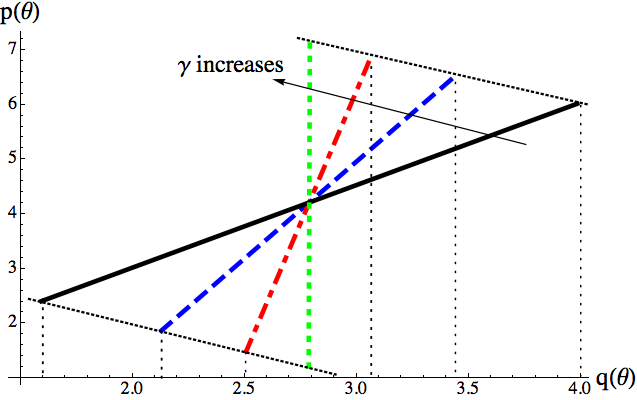
\includegraphics[width=10.cm]{figch1/monopoly_complet.png}\label{monopsup}}\quad
\subfigure[\small{$S^{-1~*}(p)$}]{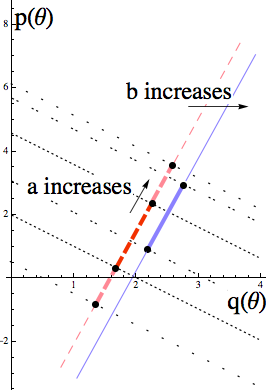
\includegraphics[width=4.5cm]{figch1/monopoly_completab.png} \label{monopab}}}
\captionsetup{singlelinecheck=off}
\caption[Static symmetric oligopoly]{\small{ \textbf{\subref{monopsup}} Four optimal supply schedules are plotted. In black (full line) $\gamma=0$. As $\gamma$ increases we transition from the black curve to the blue curve (large dashes), then the red curve (mixed dashes) and then finally for $\gamma\to\infty$ to the green one (small dashes). The range of production is highlighted for each curve through the thin vertical dotted lines. 
\vspace{0.1cm}

\textbf{\subref{monopab}} The thin black dotted lines represent the extremal demand functions given $a$ and $b$, i.e. $D(\underline{\theta},p)$ and $D(\overline{\theta},p)$. In red (dashed) the solution for a given value of $b$. As $a$ increases, the solution widens from the thick deep red region to the thick light red one. In the case for which $a$ is kept constant and $b$ is increased the solution shifts from the dashed deep red region to the full thick blue one.   
}} 
\label{fig:monop}
\end{figure}

\section{The Symmetric Oligopoly}\label{oligosolve}

We keep the same linear demand specification as in the monopoly, therefore, with $n$ competitors one has to consider the residual demand faced by each producer: 
\begin{flalign}
&S(p(\theta))=a\theta+b-(n-1)S(p(\theta))-p&\label{condsymi}\\
&S(p(\theta))=\frac{a\theta+b-p}{n} &\label{supequ}\\
&S'(p(\theta))=\frac{a-\dot{p}}{n\dot{p}}&\\
&S''(p(\theta))=-\frac{a\ddot{p}}{n\dot{p}^3}&\label{condsymf}
\end{flalign} 
For concision, we drop the explicit dependencies of the different functions on their arguments in the following equations; $f(\theta)$, $p(\theta)$ and $S(p(\theta))$ will be noted $f$, $p$ and $S$ respectively. The maximization program now writes:
\begin{equation}
%\begin{split}
\displaystyle{\max_{p(\cdot)}}~\int_{-1}^{1} f\bigg(p(a\theta+b-p-(n-1)S) -\frac{\lambda}{2}(a\theta+b-p-(n-1)S)^2%\\
-\frac{\gamma}{2}(1-\theta^2) \left(a-\dot{p}(1+(n-1)S')\right)^2\bigg)d\theta
%\end{split}
\label{maxoligopo}
\end{equation}
\begin{eqnarray}
s.t.\hspace{2cm}&\dot{p}\in[0,a] \nonumber\\
&p\leq a\theta+b \nonumber
\end{eqnarray}
with, as before, $\dot{X}=\frac{dX}{d\theta}$ and $X'$ is the derivative of function $X$ with respect to its argument. 

\subsection*{Results}
\begin{proposition}\label{propoligo1}
The solution exists, is unique, and has the following form:
\begin{equation}
\forall \theta \in [-1,1],~p^*(\theta) =aK_1\theta+bK_2 \label{oligosol}
\end{equation}
with 
\begin{flalign}
&\displaystyle{K_1=\frac{n\sqrt{(4\gamma+\lambda+n)^2-4n+4}-(4\gamma+\lambda+n)(n-2)}{2(4\gamma+\lambda+2n)}}& \\
&\displaystyle{K_2=\frac{\lambda(n-1)+K_1(\lambda+n)}{(\lambda+n)(n-1)+K_1(\lambda+2n)}}&
\end{flalign}
and the supply schedule has the following expression:
\begin{flalign}
&S^*(p)=\frac{1}{n}\left( p\left( \frac{1}{K_1}-1\right)+b\left( 1-\frac{K_2}{K_1}\right) \right)&
\end{flalign}
\end{proposition}
\begin{proof}
 See Annex \ref{annex1}. \qed
\end{proof}

\begin{proposition}\label{oligoslope_prop}
The slope of the supply schedule is increasing with $\gamma$ and the schedule is shifted to the right of the plane $(q,p)$ as $\gamma$ increases. This is to say that the schedule rotates around a point in the positive quadrant of the plane. 
\end{proposition}
\begin{proof}
See Annex \ref{oligopslope_proof}. \qed
\end{proof}

We are now going to focus on the graphical representation of these solutions. As in the monopoly case we obtain unique solutions of increasing steepness in the ramping cost parameter $\gamma$. When the ramping costs increase, it becomes more and more costly to allow for a large domain of potential quantities to be produced. \\

The black curve in Fig.~\ref{fig:oligop} corresponds to the limit solution when $\gamma\to0$, for which the problem gets closer to that of KM, i.e. no ramping costs. Note that as long as $\gamma\neq0$ the solutions are unique. This contrasts with the case of $\gamma=0$ which is the model presented in KM, for which there is a continuum of solutions. There is no smooth transition between our sets of solution: when considering ramping costs, there is a single Nash equilibria, even in the limit of small such costs.\\

Secondly, in their paper, Klemperer and Meyer show that in the limit of a diverging upper bound for their shocks, their continuum of solutions converges towards a unique solution. Our unique solution in the limit of small ramping costs is the same as that ok KM in the limit of infinite support of demand shocks.\\

\begin{proposition}
When $\gamma\to0$, the solution remains unique and converges towards the linear schedule available in KM's set of solutions, that is the same schedule selected with KM's selection rule obtained when considering an infinite support for the shocks.
\end{proposition}
\begin{proof}
It is straightforward to check that $K_1$ and $K_2$ have the same values as KM for $\gamma\to0$. \\
More intuitively the argument is as follows. When $\gamma\to 0$, with $\gamma>0$, we retain a unique solution although the problem itself converges towards that of KM. When $\gamma = 0$, we are back to the KM situation with a continuum, however we can come as close to 0 as we want while maintaining a unique solution. We should therefore select an equilibrium present in KM's continuum. When KM take the limiting case of an infinite support of shocks they select a unique equilibrium. In our case we can do the same thing by taking $a\to\infty$. In the limit, our solution being in their set which converges to a unique equilibrium, those two selected equilibria should be equal. Now note that our solution does not depend explicitly on $a$ so that when the support is finite, we still select the same equilibria out of what is now a continuum of equilibria in KM's framework.             \qed
\end{proof}


\begin{figure}[h] 
\centering
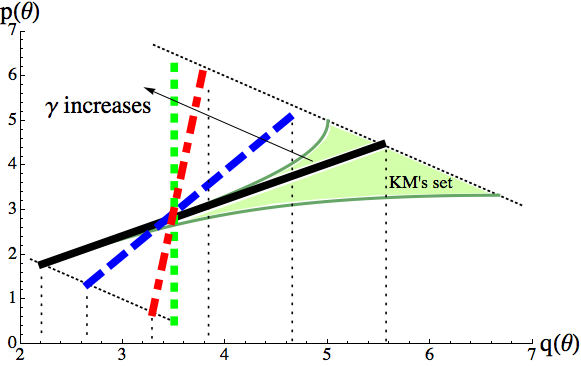
\includegraphics[width=12cm]{figch1/oligovraiKMd.png}
\caption{\small{This graph plots $S^*(p)$ for different values of the ramping cost parameter, and compares them to the set of equilibria obtained in KM's framework. Four optimal supply schedules are plotted. The black curve (full line) corresponds to the case where $\gamma\to0$. As before, as $\gamma$ increases the optimal schedules get steeper and steeper until in the limit of $\gamma\to\infty$, the optimal schedule attains a vertical slope. In addition, we show the set of available equilibria in KM's model in light green, and the extremal demand schedules in dashed black.  }} \label{fig:oligop}
\end{figure}

Intuitively, as we take $\gamma$ to $0$ we come closer to the situation captured in KM, but as long as $\gamma>0$, the producer still faces ramping costs, and therefore converges towards the only linear schedule available in KM's set, as shown in Fig.~\ref{fig:oligop}, in which we plot our solutions on top of KM's solution set in order to clarify the comparison. \\

Note that it isn't possible to transition smoothly from our model to that of KM, although they are obviously closely related. Indeed, $\forall \gamma>0$, our model yields unique solutions, but for $\gamma=0$ we return to KM's model for which there is a continuum of equilibria. There is an intrinsic discontinuity between these two models, namely, the correspondence $\Gamma(\gamma)$ associating the set of equilibria to the symmetric oligopoly problem obtained for a given value of the ramping cost parameter $\gamma$ is not lower hemicontinuous at $\gamma=0$. \\

In addition to proposing a way to take into account dynamic technological constraints, our model provides a selection rule to choose from the continuum of equilibria described in KM's seminal work, i.e. the solutions' stability to ramping costs.\\

\begin{proposition}\label{oligoequilibrianeg}
With $\gamma > 0 $, their exists values of shocks for which the prices are negative. More precisely, their exists negative prices if the following condition on the parameters of the shocks holds:
$$b\frac{K_2}{K_1}<a<b(1-K_1)$$
\end{proposition}
\begin{proof}
The method is exactly the same as that used in prooving proposition \ref{monopequilibrianeg}, noting that $(K_1, K_2)\in (0,1)^2$. \qed
\end{proof}

As in the monopoly case, we have the property that there exists situations in which our model can exhibit negative prices. This is interesting because negative prices are observed on the electricity market, and is often described as a way for non-flexible committed producers to subsidize consumption in order to avoid reducing production too much.\\

To sum up, we have here a model whose solutions depend on the distribution of shocks, therefore we are able to capture the interday variation of bids by assuming that the distribution of shocks varies from day to day. In this case, there exists only one symmetric equilibria each day, function of the distribution of shocks.\\

\subsection{Discussion}

This result sheds some light on one of the questions that the electricity market literature focuses on. \\

Accounting for ramping costs induces a collapse of the equilibria set from a continuum to a unique element. \\

Most of the tacit collusion concern that is present in the literature is based on the existence of a continuum of solutions \cite{bolle1992supply}. This continuum is thought as being conducive of tacit collusion because the electricity market entails repeated interactions between producers. In this case, producers can be feared to be able to learn to pick the most profitable Nash equilibria. Although a Nash equilibrium is not usually considered conducive to collusion, as each player's strategy is the best response to the other's and there is no profitable deviation, a multiplicity of Nash equilibrium lets open the possibility to pick and choose the most profitable one out of the available options, as compared to the one leading to the strongest competition.\\

Our result implies this pathway for tacit collusion is not available anymore. With only one Nash equilibria at any given time no learning can bring about tacit collusion. This is a strong result about the structure of competition in our framework. The existence of ramping costs leads to a model in which no tacit collusion can exist, suggesting that the policy recommendations about such collusion stemming from the supply function equilibria litterature might be strongly dependent on not taking into account ramping costs.\\

Our solutions are also not ex-post optimal contrary to the traditional results. As our solutions depend explicitly on the structure of the uncertainty around demand shocks, any additional information shifting the expected distribution of shocks would imply a different bid. Ex-post optimality is a very strong result, and, one could argue, more of a quirck from the usual models than its abscence in ours.\\

We are also able to account for negative prices which was impossible in the previous framework. Such negative prices are actually observed, although rarely, on the market: producers prefer to subsidize consumption instead of decreasing production by a lot. In our framework, if the ramping costs are large enough, and the demand shocks can reach a small enough value, our solutions can yield negative values: the equilibrium price might even be below the marginal cost of production, understood here as $\partial_q C$ which by definition does not capture our ramping costs.\\

%
%In addition to this consideration, one must note that our unique solution rotates towards a steeper and steeper supply schedule as the ramping costs increase. However this rotation does not occur around the mean demand shock, but around a lower shock value. This means that, in expected terms, our solutions are more costly than the one selected by KMs infinite support argument. As long as the ramping costs are not too high, our solution lies in the region of the price quantity plane delimited by the continuum of solutions of KM. Therefore, for empirical work trying to estimate

In the next section we are going to present how to capture richer dynamics, and especially how the surface of bids should evolve with time when the producers have information about the anticipated variation of shocks during the day. 

\section{Dynamic behavior of the bids} \label{dynamics}
The classical supply function equilibria models, as described before, yield a continuum of Nash equilibria, and each one of those equilibria is ex-post optimal. This a very strong result that we are going to take some time to describe and comment.\\

Consider for a moment that firms competing in supply schedules reach one of the many possible Nash equilibria under such a setup, and that they commit to their schedules. Now consider that the firms face a succession of demand shocks, and that this yields a succession of market outcomes. As the Nash equilbria are ex-post optimal, it means that given the strategies played by the other firms, no firm has any regrets concerning its strategy. Knowing about the realized demand shocks does not imply any willingness to change strategy as long as other firms keep their strategies fixed, and as long as the support of shocks is not reduced ot a point (one could think of observed realizations of shocks as helping to narrow down the expected range of shocks without implying a pinpoint accuracy).\\

A corollary to this observation is that the distribution of anticipated shocks does not play any role in KM's paper, apart from its bounds. Knowing that the demand shocks are going to be drawn from distributions of high or low values does not affect the willingness to play a given strategy, as long as the support does not evolve. The little role that is played by information about shocks in KM's paper is even more counter-intuitive: to a certain extent, information about demand shocks gives rise to a larger continuum of solutions. Indeed, if one compares the equilibria available to firms for a given support $\{\theta\}_1=[\underline{\theta}_1, \overline{\theta}_1]$, noted ${S^*}_1$, to those obtained for a support strictly included in the first one $\{\theta\}_2=[\underline{\theta}_2, \overline{\theta}_2]\subset\{\theta\}_1$, noted ${S^*}_2$, then the set of equilibria will be larger in the second case, in the sense that $ {S^*}_1\restriction_{\{\theta\}_2}\subset {S^*}_2$ (where $\restriction_{\{\theta\}_2}$ denotes that the supply functions are restricted to values over $\{\theta\}_2$). \\

However, actual firms bidding on the electricity markets are known to be actively engaged in forecasting the future demand levels in order to build their strategies. Bids that we can observe on the electricity markets change from hour to hour even when demand does not vary enough to warrant a change of online plants, a consideration that could explain some of the supply schedules variations. \\

The general interpretation of KM's paper when applied to electricity markets is that for some unknown underlying process, strategies converge towards different equilibria of the set of available equilibria from hour to hour. One can note that the general intuition for strategies converging towards Nash equilibria in the first place is through either a high degree of sophistication on the part of firms, or through a more organic learning process. Neither of these two explanations can account for frequent switching from one Nash equilibria to another, out of a myriad of available options, wihtout considering some communication among firms. Furthermore, if such communication existed, it should be expected to yield the most profitable equilibria out of the available lot.\\ 

We think that this strand of argument trying to explain bids' dynamics in the light of the supply function equilibria framework is unsatisfying and we argue that forecasting demand becomes important for firms when one considers dynamic effects, that is effects that are history dependent, of which ramping costs which we model in this paper are an instance (one can think of start-up and shut-down costs as another instance of such dynamic effects). \\

The model described in the previous section doesn't account for these hourly dynamics. Here we present a way to capture these intraday variations, by considering bids that depend continuously on the time $t$. We will show that our results imply that firms are not oblivious to information about the distribution of shocks anymore, and more than that, that their strategies directly evolve with the evolution of their knowledge about uncertain furture shocks.\\


\subsection{The setup}\label{setupdyn}
Previously, the SDE (stochastic differential equation) defining the dynamics of the problem was written as: 
$$d\theta(t)=-2\theta(t) dt+\sqrt{1-\theta(t)^2}dB_t$$ 
This specification implied a stochastic trajectory for the shocks, bounded by a constant envelope. That is to mean that, lacking any knowledge of the value of the shock at a point in time close to the period under consideration, the distribution of shocks does not depend on time.\\

To account for these intraday variations we are going to define a richer SDE, a non-stationary one. \\

SDEs have been well studied and as a consequence there exists a number of families of SDEs satisfying numerous characteristics \cite{enveloppe}. The goal here is to find one SDE that will allow us to capture some of the dynamics of shocks and how this might influence strategies, while keeping it as simple as possible. Just as in the previous section, the first caracteristic that we want is to consider SDEs that imply a bounded support of shocks. This restricts our possible choice to four families out of the classical ones: Generalised Beta I, Beta, Power, Uniform. We also consider that a desirable property is that the distribution reaches 0 continuously at the bounds of its support, because there is no boundary condition on the demand for electricity that would justify that one has a positive probability of reaching a given bound, but a zero probability of reaching an infinitesimally close value to this bound. This restricts us further to only two families: Generalised Beta I and Beta. For tractability reasons we will focus here on the Beta family of SDEs, and more precisely on one of the simplest Beta SDE. However, we want to note that this choice stems from our focus towards solving analytically the problem at hand and obtain closed form solutions. If one were to try and estimate the distribution of shocks anticipated by firms from market data one might want to try and find which of the Beta or Generalised Beta I SDEs might match the distribution of errors between the published day -1 estimates for demand and the observed quantities.\\

Define the evolving envelope of shocks by two functions, $(\underline{\theta}(t),\overline{\theta}(t))$, respectively the lower and upper bounds of the shocks. These two functions, although very easy to comprehend, are not the most useful way to define the boundary. Instead we are going to use the average value of the shocks, and the half width of the envelope, $(\hat{\theta}(t), \omega(t))$. This means that $\underline{\theta}(t)=\hat{\theta}(t)-\omega(t)$ and $\overline{\theta}(t)=\hat{\theta}(t)+\omega(t)$. The only restriction we impose on the envelope is that we require it to be continuously differentiable, that is $(\hat{\theta},\omega)\in\mathcal{C}^1(\mathbb{R})$.\\

Consider the following SDE which is the simplest Beta SDE that we can pick that still allows us to have a free choice of the bounds of shocks. We want the simplest possible form to make it possible to obtain closed form solutions, yet still account for free dynamics of the bounds. For readability, we drop the explicit dependency of the different functions on time, that is $\theta(t)$, $\hat{\theta}(t)$ and $\omega(t)$ will be noted $\theta$, $\hat{\theta}$ and $\omega$:
\begin{equation}
\begin{split}
  d\theta=\left[(\hat{\theta}-\omega-\theta)+\left(1+\frac{1}{\omega}\frac{d\omega}{dt}\right)(\hat{\theta}+\omega-\theta)+\left(\frac{d\hat{\theta}}{dt}-\frac{d\omega}{dt}\right)\right]\cdot dt\\+\sqrt{\left(1+\frac{1}{\omega}\frac{d\omega}{dt}\right)(\theta-\hat{\theta}+\omega)(\hat{\theta}+\omega-\theta)}\cdot dB_{t}
\end{split}
\end{equation}

The distribution of the shocks can be obtained through Fokker-Planck's equation \ref{FokP} and we obtain:
\begin{equation}
f(\theta,t)=\frac{3}{4\omega(t)^3}(\theta(t)-\hat{\theta}(t)+\omega(t))(\hat{\theta}(t)+\omega(t)-\theta(t))
\label{distrib_prerescale}
\end{equation}

In the following analysis, we are going to rely on the fact that the term $\left(1+\frac{1}{\omega}\frac{d\omega}{dt}\right)>0$. The justification for this inequaliy comes from the following remark: if one were to rescale time in the above equations, there wouldn't be any explicit change in the equilibrium distribution \ref{distrib_prerescale}. The only effect that such a rescaling would play is in the variance of the Brownian term. In order to insure that our inequality is correct, one has to make sure that the variation of the envelope term occurs on longer timescales than the characteristic timescale of fluctuations in our problem, that is the timescale that fixes the rate at which information leaks out of the knowledge of the value of one shock at a given point in time. We are trying to capture the hourly changes in firms strategies when demand fluctuates at higher frequencies (think of the collection of individuals that choose to switch lights on or off at any given point in time in an entire country for instance). We therefore consider that this assumption is sound in this situation.\\

More formally, one can define $\tau$ a rescaling parameter allowing to change the rate at which the brownian process blurs information pertaining to an initial condition. We rescale time using this parameter, so that time $t$ and the rescaled time $t_r$ verify $t_r=\tau t$. \\

We can rewrite the above equations as:
\begin{equation}
\begin{split}
  d\theta=\left[(\hat{\theta}-\omega-\theta)+\left(1+\frac{\tau}{\omega}\frac{d\omega}{dt_r}\right)(\hat{\theta}+\omega-\theta)+\tau\left(\frac{d\hat{\theta}}{dt_r}-\frac{d\omega}{dt_r}\right)\right]\cdot dt_r\\+\sqrt{\left(1+\frac{\tau}{\omega}\frac{d\omega}{dt_r}\right)(\theta-\hat{\theta}+\omega)(\hat{\theta}+\omega-\theta)}\cdot dB_{t_r}
\end{split}
\end{equation}

and 

\begin{equation}
f(\theta,t_r)=\frac{3}{4\omega(t_r)^3}(\theta(t_r)-\hat{\theta}(t_r)+\omega(t_r))(\hat{\theta}(t_r)+\omega(t_r)-\theta(t_r))
\label{distrib_postrescale}
\end{equation}

By assumption, $\tau$ is small enough for the loss of information due to the stochastic nature of the process to be faster than the typical timescale of variation of strategies, therefore by hypothesis $\left(1+\frac{\tau}{\omega}\frac{d\omega}{dt_r}\right)>0$ is valid. We will drop this rescaled time index in the following sections as equations \ref{distrib_prerescale} and \ref{distrib_postrescale} are equal, it was just a temporary definition to justify the sign of the term that depends on the time derivative of the envelope. We will keep this $\tau$ parameter explicit however, in order to allow discussions differentiating effects related to the speed of variation of the envelope or to the relative timescales of this variation and the underlying stochastic process.

\subsection{Results}
\subsubsection{Dynamics in the case of the Monopoly and of the oligopoly}
We start by describing the dynamics of the monopoly case because the oligopoly case is not richer dynamically, but it is more complex to describe. \\

Our stochastic maximization program can thus be rewritten as a regular optimal control problem as in section \ref{monosolve}, but taking into account the time depency: 

\begin{equation}
\displaystyle{\max_{S_i(p,t)}}~\int_0^T\int_{\underline{\theta}(t)}^{\overline{\theta}(t)} f(\theta,t)\left(p(\theta,t)S_i(p(\theta,t),t) -C_s(S_i(p(\theta,t),t))-\frac{\gamma}{2}\sigma(\theta,t)^2\left(S_i'(p(\theta,t),t)\dot{p}(\theta,t)\right)^2\right)d\theta dt
\end{equation}
\begin{eqnarray} 
s.t.\hspace{2cm}&S_i'(\cdot)\geq0 \nonumber\\
&\dot{p}\geq0\\
&D(\cdot,\cdot)\geq0 \nonumber\\
\end{eqnarray}


\begin{proposition}\label{monopropdyn}
In the case of an envelope evolving with time, that is shocks belonging to the bounded support $[\hat{\theta}(t)-\omega(t),\hat{\theta}(t)+\omega(t)]$, there exists a unique optimal solution to the monopoly problem. It can be expressed as as surface in the price-quantity-time space:
\begin{flalign}
&p^*(\theta(t),t)=\frac{4\gamma\left(1+\frac{\tau}{\omega}\frac{d\omega}{dt}(t)\right)+1+\lambda}{4\gamma\left(1+\frac{\tau}{\omega}\frac{d\omega}{dt}(t)\right)+2+\lambda}\cdot\theta(t)-\frac{1+\lambda}{2+\lambda}\cdot\hat{\theta}(t)&\label{monopdynp}
\end{flalign}
The corresponding optimal supply schedule writes as:
\begin{flalign}
&S^*(p, t)=\frac{1}{4\gamma\left(1+\frac{\tau}{\omega}\frac{d\omega}{dt}(t)\right)+1+\lambda}\left(p(t)+\frac{4\gamma\left(1+\frac{\tau}{\omega}\frac{d\omega}{dt}(t)\right)}{2+\lambda}\cdot\hat{\theta}(t)\right)&\label{monopdynS}
\end{flalign}
$\forall p(t)\in[p(\hat{\theta}(t) - \omega(t),t), p(\hat{\theta}(t) + \omega(t),t)]$
\end{proposition} 
\begin{proof}
See Annex \ref{monopdyn_proof}.  \qed
\end{proof}

Note that if $\frac{d\omega}{dt}=0$ equations \ref{monopdynp} and \ref{monopdynS} are equal to equations \ref{monopsol} and \ref{monopS} respectively as expected. Note also that the solution is exactly the same as in the static monopoly case in which one replaces the ramping cost parameter $\gamma$ by $\gamma\left(1+\frac{\tau}{\omega}\frac{d\omega}{dt}(t)\right)$. This surprising fact, that our dynamic optimal strategy is simply a naive version of the static one with a specified dynamic stochastic process, can be understood as a consequence of the assumptions we have had to make in section \ref{sec_ramping_costs}. \\

That is because in section \ref{sec_ramping_costs}, in Annex. \ref{stochasticdyn_proof} in which we develop the argument in more detail, and in section \ref{setupdyn} we end up in effect making a scale separation argument: the ramping costs are completely driven by the very short term fluctuations, whereas the evolution of these ramping costs is driven by the longer timescale at which our information about the demand shocks evolves over time. This means that we make a version of what physicists call a quasi-static argument: because of this time-scale separation between what drives our ramping cost and our information about the shocks, we can effectively reason in two steps, first solving for the static situation, and then injecting naively the slow changes in the static results with confidence as to the validity of this approximation as long as the assumption about this separation of scale is verified.\\

The consequence of this is that we have a dynamic version of our static oligopoly of the same nature as for the monopoly above.\\


\begin{proposition}\label{oligodynp}
The solution exists, is unique, and has the following form:
\begin{equation}
\forall \theta \in [-1,1],~p^*(\theta) =aK_1(t)\theta+bK_2(t) 
\end{equation}
with 
\begin{flalign}
&\displaystyle{K_1(t)=\frac{n\sqrt{\left(4\gamma\left(1+\frac{\tau}{\omega}\frac{d\omega}{dt}\right)+\lambda+n\right)^2-4n+4}-\left(4\gamma\left(1+\frac{\tau}{\omega}\frac{d\omega}{dt}\right)+\lambda+n\right)(n-2)}{2\left(4\gamma\left(1+\frac{\tau}{\omega}\frac{d\omega}{dt}\right)+\lambda+2n\right)}}& \\
&\displaystyle{K_2(t)=\frac{\lambda(n-1)+K_1(t)(\lambda+n)}{(\lambda+n)(n-1)+K_1(t)(\lambda+2n)}}&
\end{flalign}
and the supply schedule has the following expression:
\begin{flalign}
&S^*(p,t)=\frac{1}{n}\left( p\left( \frac{1}{K_1(t)}-1\right)+\hat{\theta}\left( 1-\frac{K_2(t)}{K_1(t)}\right) \right)&\label{dynsupply}
\end{flalign}
\end{proposition}
\begin{proof}
 See Annex \ref{oligodyn_proof}.\qed 
\end{proof}

\subsection{Discussion}

In both situations, the optimal supply schedule is shifted uniformly following the expected shock $\hat{\theta}(t)$, which is a rather intuitive result: if on average demand shifts upwards, the producers want to extract more profit and shift their supply curve accordingly, but there is no reason to change slope.\\

What is less trivial is the way the slope behaves. Let us focus on the monopoly result for a start. The slope is affected as if the ramping cost parameter was fluctuating with the relative change in the width of the bounds of the shocks (term in $\frac{1}{\omega}\frac{d\omega}{dt} $). The transition between a low uncertainty region to a higher uncertainty one behaves as if during the transient regime the ramping cost parameter had a higher value, implying a higher slope. \\
         
The optimal supply schedule depends on the relative rate of change of the width $\frac{1}{\omega}\frac{d\omega}{dt}$ and on the average shock $\hat{\theta}$. More precisely, with a constant width, the optimal supply schedule varies according to variations in the expected average value of the shocks. This is quite standard, if demand is higher, the price and quantities both increase, and here this increase occurs with a constant slope. The behavior of the supply schedule when the width varies is less trivial. \\

Remember that when describing the slope of the schedule, we are considering the plane $(quantity, price)$ while the schedule as defined by $S^*(p)$ represents the same curve but in the plane $(price, quantity)$. An increase in width is equivalent to a higher ramping cost parameter while a decrease in width is equivalent to a lower ramping cost parameter. These results are illustrated in Fig. \ref{figdyn1}. \\

To understand the economic intuition behind this result, consider first an increase in the width of the envelope on the graphic on the right, the uncertainty level given by the orange line. At this point in time, the uncertainty is increasing, therefore the shocks are going to be larger, the variations in demand too, and to face this increase, the slope is larger so as to reduce this expected increase in ramping costs. In the case of the green line, the uncertainty is decreasing, the ramping costs incurred are expected to decrease, thus this constraint being relaxed the slope can reduce to extract more profit through more variations in quantity than if the slope had remained high.\\

One can contrast this behaviour to the one described on the left hand side of the figure, where the uncertainty is constant, but the average shock is not. This implies only a vertical translation of the curve, without changes in the slope. Here the slope is fixed by a given level of uncertainty, to exploit an increased demand, the supplier simply increases its prices, but it doesn't need to hedge against increased variation by encouraging or discouraging variations in quantity by playing with the slope.\\


% Consider now one possible value of $\theta(t_1)$. At $t_1+dt$, had the width been constant there would have been a given level of uncertainty about the values that $\theta(t_1+dt)$, and thus the ramping costs, could have taken.  If the width of the envelope is increasing then there is more uncertainty regarding the potential values that could be taken by $\theta(t_1+dt)$, therefore more expected ramping costs incurred, and a higher slope to hedge these costs. On the other hand, when the width decreases, the situation is reversed. In that case, we move towards a situation in which there is less uncertainty about the ramping costs, so that the slope is smaller than for a constant envelope. This difference between increasing and decreasing width is illustrated by comparing the two regions of the envelope displayed in (full) black line in Fig. \ref{figdyn1}. In addition, when contrasting the left and the right side of the figure one sees that the change in the informativeness of the envelope is captured by the relative change of the width: for the same rate of change, if the width is larger (right) then the change in informativeness is smaller (the change in the area captured by the (dashed) red and (full) green arrows).  \\

\begin{figure}[h] 
\centering
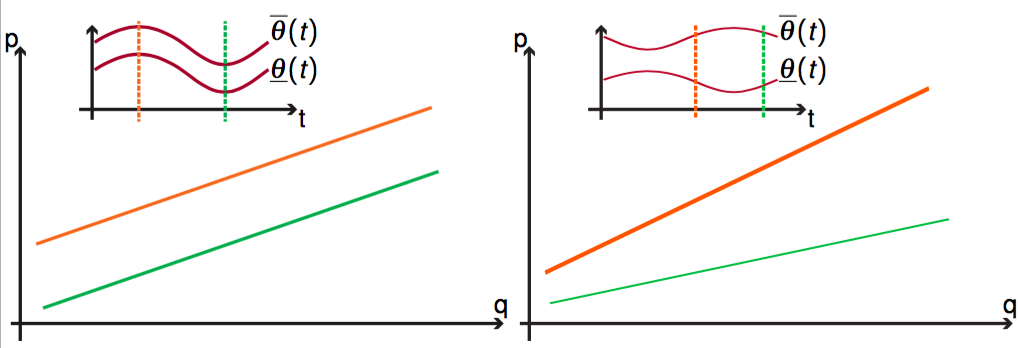
\includegraphics[width=15cm]{figch1/uncertainty.png}
\caption{\small{On the left, this graph plots an envelope of constant width $\omega(t)$ but varying average. The insert represent this envelope, while the graph itself represents the supply curves associated with the points in time represented by the green and orange dotted lines on the insert. On the right, this graph plots an envelope of constant average but varying width $\omega(t)$. }} \label{figdyn1}
\end{figure}

All of this reasoning applies to the dynamic oligopoly result as well as the effect can be understood in the same way as for the monopoly: changes in the width of the shock's bounds behave as if there was an effective dynamic cost that was higher than the baseline when information about the shocks is lost, and lower than the baseline when information is gained.

\section{Limits}\label{limits}

This section aims at discussing whether or not one can consider that the mapping of these results on the real world is a set of non zero measure, to put it bluntly.\\

Further avenues of research would be to generalize our results to larger classes of demand functions. One could also solve the static case for different SDE's in order to test the sensitivity of our results on the underlying "mechanics" of the stochastic process. This has also been pursued without conclusive results: solving the optimization problem becomes quickly extremely difficult, as the second order differential equations exhibit poles, and divergences are difficult to cope with in optimization problems. \\

The nature of these avenues of research is testament to the fact that our results are obtained for a very narrow setting, one chosen to obtain closed form formulas. However, although a healhty dose a skepticism as to the applicability of the closed form formulas is therefore warranted, I would like to argue that the results hint towards at least one more general takeaway message, namely the collapse of the set of equilibria.\\

This result stems from the nature of the mathematical problem and not from the way we set up the problem in order to maximize our chances of closed-form success per se. Therefore I think it hints towards possible more general results. The problem is the complexity of the maths as soon as one deviates from the simplest version of the problem presented here. \\

The question then becomes one of the method to employ to obtain those results. There is one tool that might prove useful: numerical simulations. One can solve the differential equations involved here numerically, check ex-post whether they satisfy the other conditions, and in so doing provide boundaries around possible solutions. If the unicity is a characteristic that is indeed more general than our model here, there is 0 probability of finding such a solution by the method proposed, quite literally. However providing such bounds, although not demonstrating the existence of a solution, could provide circumstantial evidence towards such a result.\\

More generally, I think numerical methods as a guide for theoretical results have not been exploited to their fullest.  

\section{Concluding Remarks}\label{ccl}

In this chapter we have introduced a supply function equilibria model of ramping costs under uncertainty.\\

By introducing technological constraints previously neglected we are able to take into account the effects of the dynamics of demand shocks on the supply function framework. We restrict ourselves to linear demand. The optimal supply schedules obtained are unique. This is a striking result when compared to traditional multiplicity of equilibria. Although we do not solve the model in the case of a general demand function, we think that our results make a strong case for the reduction of the set of equilibria, in our case to a unique equilibrium, when taking into account dynamic effects, that is strategies that are history dependent. \\

We introduce a mathematical toolbox that was absent from this litterature in the past, and notably classes of stochastic differential equations that can be used to pick and choose processes yielding specific closed form distributions of probability of shocks at equilibrium. \\

Our methodology further introduces the notion of time-scale separation to our problem, which allows to transcribe quite simply static solutions to the case of dynamic envelopes of shocks, as long as the static case is solved for the same functionnal form of stochastic processes. In our case we focus our study to quadratic distributions, which we then extend to cope with any functional form for the time dependency of the envelope of shocks.\\

Our results are congruent with the economic intuition one can have about ramping costs: when they increase, the slope of the supply schedule increases in order to reduce the range of variation in production for a given range of variation of demand shocks.\\

Although mathematically more demanding than the traditional model by Klemperer and Meyer, we consider that this new model, while conceptually sparing (we only add ramping costs) allows for a richer, more realistic description of the electricity market, and opens new research avenues.  It yields precise and testable predictions on the dynamics of the electricity market with tractable functional forms, at least in the linear demand case. \\

In addition, by explicitly modeling the dynamics, our work opens the possibility to explore interactions between intraday and day-ahead markets, markets that were indistinguishable in the previous framework, which explains why the analysis of the interaction between different ways to trade elecrticity focused on day-ahead markets and forward contracts: if solutions are ex post optimal, there is no need to create a second type of spot market, with a shorter time horizon, the bids of the previous day should suffice. \\

Further avenues of research would be to generalize our results to larger classes of demand functions. As hinted in the text of this chapter, a lot of effort has been invested towards this goal without results unfortunately. One could also solve the static case for different SDE's in order to test the sensitivity of our results on the underlying "mechanics" of the stochastic process. This has also been pursued without conclusive results: solving the optimization problem becomes quickly extremely difficult, as the second order differential equations exhibit poles, and divergences are difficult to cope with in optimization problems.\\

Finally, and more generally, we think that this concept of ramping costs, the fact that change is costly, is ubiquitous and could fuel interesting research into the dynamics of a large range of markets. Such avenues have been pursued in the case of stochastic optimal control, that is, instantaneous reactions to stochastic shocks. Here we are describing a market on which agents are forced to optimize in advance, so that they have to react to continuous changes in the anticipated shocks, but not the shocks themselves, which can be understood as stochastic optimization with periodic commitment. \\

The goal of the second and third chapter is to test these theoretical predictions on French day-ahead data. The next chapter focuses on building methods to be able to perform such tests in the third chapter. As the actual supply schedules are not linear, we need to be able to define their local slopes and to define points that can be compared to one another across schedules. We also describe how we build the different controls that need to come into play to estimate properly the impact of uncertainty on the slope, but more importantly we introduce one class of uncertainty estimates associated with weather. With these elements in place, we have a way to compare schedules to one another, and to estimate uncertainty for a given schedule, and therefore look into the effect of uncertainty in the third chapter. 

%\bibliographystyle{te}
%\bibliography{biblio}
\newpage
\begin{subappendices}
\section*{Appendix}
\addcontentsline{toc}{chapter}{Appendix}
\numberwithin{figure}{section}
\numberwithin{equation}{section}

\section{Proof of equation \ref{markovtimedep}}\label{stochasticdyn_proof}
We are here going to detail how we obtain the result in equation \ref{markovtimedep} on which the proofs of our dynamic results rely heavily. Recall that we are computing the continuous time limit of our ramping cost term which can be quite simply defined in the case of discrete dynamics but for which one has to work a bit more in order to cope with the non differentiable nature of stochastic processes. \\

We are therefore going to first consider the discrete case of a random walk of timestep $\Delta t$ which converges towards the It\={o} process \ref{sdegen}, using the Euler-Maruyama approximation, a generalization of the Euler method to stochastic differential equations. We consider a Markov chain $Y$ defined as follows: 

\begin{equation}
\Delta Y_n=Y_{n+1}-Y_n= \mu(Y_n,n \Delta t)\Delta t+\sigma (Y_n,n \Delta t)\Delta B_n
\end{equation}


We want to derive the following: 
\begin{footnotesize}
\begin{eqnarray}
\lim_{\Delta t \to 0}\mathbb{E}\left[\frac{\Gamma(\Delta t)}{2}\left(\frac{\Delta S_i(p(\theta(t),t),t)}{\Delta t}\right)^2\middle \vert \theta(t)  \right] &=& \frac{\gamma}{2} (\partial_1S(p(\theta(t),t),t)\partial_1p(\theta(t),t))^2 \sigma(\theta,t)^2
\end{eqnarray}
\end{footnotesize}

Let us first compute the first order expansion of $\Delta S_i(p(Y_n,n\Delta t),n \Delta t)$, by assuming that both $S_i$ and $p$ are continuously differentiable with respect to their arguments:
\begin{small}
\begin{eqnarray}
\Delta S_i(p(Y_n,n\Delta t),n \Delta t) &=& \frac{\Delta S_i}{\Delta p}\left( \frac{\Delta p}{\Delta Y}\frac{\Delta Y}{\Delta t}\Delta t+ \frac{\Delta p}{\Delta t}\Delta t\right) + \frac{\Delta S_i}{\Delta t}
\Delta t +\mathcal{O}(\Delta t^2)
 \end{eqnarray}
 \end{small}
Using our differentiability assumption, note that the terms that do not depend on $\Delta Y$ scale with $\Delta t$, and that the term depending on $\Delta Y$ cannot be grouped in the same way, due to its stochastic nature, therefore:
\begin{small}
\begin{eqnarray}
\frac{\Delta S_i(p(Y_n,n\Delta t),n \Delta t) }{\Delta t} &=& \frac{\Delta S_i}{\Delta p} \frac{\Delta p}{\Delta Y}\frac{\Delta Y}{\Delta t}+\mathcal{O}(1)\\
 \left(\frac{\Delta S_i(p(Y_n,n\Delta t),n \Delta t)}{\Delta t}\right)^2 &=& \left(\frac{\Delta S_i}{\Delta p} \frac{\Delta p}{\Delta Y}\frac{\Delta Y}{\Delta t}\right)^2+ C\cdot \frac{\Delta S_i}{\Delta p} \frac{\Delta p}{\Delta Y}\frac{\Delta Y}{\Delta t} + \mathcal{O}(1)
 \end{eqnarray}
 \end{small}
 with $C$ a term that does not depend on $\Delta Y$ or $\Delta t$.\\
 
Now by considering the specification of our stochastic process we know that $\mathbb{E}\left[\frac{\Delta Y}{\Delta t}\vert Y_n\right]=\mu(Y_n,n \Delta t)$ and that $\mathbb{E}\left[\frac{\Delta Y}{\Delta t}^2 \right\vert Y_n]=\mu(Y_n,n \Delta t)^2 + \frac{\sigma (Y_n,n \Delta t)^2}{\Delta t}$. 
Using the fact that $\Gamma(\Delta t) = \gamma \Delta t + o(\Delta t)$ we obtain the result of equation \ref{markovtimedep}.


\section{Proof of Proposition \ref{monopequilibria} \label{annexmonop}}
Define the following Hamiltonian: 
\begin{equation}
\begin{split}
H(p(\theta),\dot{p}(\theta),\mu(\theta),\theta)= f(\theta)\bigg( p(\theta)(a\theta+b-p(\theta))-\frac{\lambda}{2}(a\theta+b-p(\theta))^2\\
-\frac{\gamma}{2}(1-\theta^2)\left(a-u(\theta)\right)^2\bigg)+\mu(\theta) u(\theta)
\end{split}
\end{equation}
where $u(\theta)$ is the control variable defined through the following equation of motion: $u(\theta)=\dot{p}(\theta)$, $u(\theta)\in[0,a]$. We do not consider the non-negative demand constraint and will check ex-post that our solution verifies this condition. \\

Now note that:
\begin{eqnarray}
\forall\theta\in(-1,1),&\displaystyle{\frac{\partial^2 H}{\partial p^2}}=-(2+\lambda)f(\theta)<0\label{concmono1}\\
&\displaystyle{\frac{\partial^2 H}{\partial u^2}}=-\gamma(1-\theta^2)f(\theta)<0\label{concmono2}
\end{eqnarray}
The Hamiltonian is therefore strictly concave in $p(\theta)$ and $u(\theta)$. Let $(p^*(\theta),u^*(\theta))$ be an admissible pair to the problem, that is a pair such that $u^*(\theta)=\dot{p}^*(\theta)$. If there exists a continuous and piecewise continuously differentiable function $\mu(\theta)$ such that: 
\begin{flalign}
\dot{\mu}(\theta)=-\frac{\partial H}{\partial p}^*\hspace{1.65cm}\label{mupmonop}\\
\mu(-1)=\mu(1)=0 \hspace{1.13cm}& \textrm{in order for prices to be free at the boundaries}\label{monopbound}\\
\forall (\theta,u)\in[-1,1]\times[0,a],\hspace{0.17cm}& \frac{\partial H}{\partial u}^*(u^*(\theta)-u)\geq0\label{mangaham}
\end{flalign}
with $\frac{\partial H}{\partial u}^*=\frac{\partial H}{\partial u}(p^*(\theta),u^*(\theta),\mu(\theta),\theta)$, then the Mangasarian sufficiency theorem ensures that $(p^*(\theta),u^*(\theta))$ is the optimal solution \cite[p.105]{constraint}. Let us check that eq.~\ref{monopsol} defines the optimal solution.\\

Equation \ref{mupmonop} defines $\mu(\theta)$ up to a constant. Through direct integration we obtain: $$\mu(\theta)=3a\left( (2+\lambda)\frac{4\gamma+1+\lambda}{4\gamma+2+\lambda}-1-\lambda\right)(2\theta^2-\theta^4)+const.$$
This expression is symmetric in $\theta$ therefore by choosing the adequate value for the constant, we ensure that eq.~\ref{monopbound} is satisfied. The slope of the proposed $p^*$ is in $[0,a]$ therefore eq.~\ref{mangaham} requires $\frac{\partial H}{\partial u}$ to be null.  
\begin{eqnarray}
\forall \theta \in [-1,1],~ \frac{\partial H}{\partial u}=0\implies \frac{d}{d\theta}\frac{\partial H}{\partial u}=0\hspace{3.6cm}\nonumber\\
\textrm{i.e. }\displaystyle{\dot{u} (\theta)= -\frac{4\theta}{1-\theta^2}(a-u(\theta))-\frac{(1+\lambda)(a\theta+b)}{\gamma(1-\theta^2)}+\frac{(2+\lambda)p (\theta)}{\gamma(1-\theta^2)}}
\end{eqnarray}
It is straightforward to see that the proposed solution satisfies this differential equation, thus we know that $\frac{\partial H}{\partial u}$ is a constant and as $\mu(-1)=0$ it is in fact null. Lastly,  we see that $p^*(\theta)\leq a\theta +b$.\\

The proposed $p^*(\theta)$ therefore defines the unique optimal supply function, i.e. the parametrized curve $(a \theta +b-p^*(\theta),p^*(\theta))$.

\section{Proof of Proposition \ref{monopequilibriaKM} \label{annexmonopKM}}
Consider the following profit:
$$p\cdot D(\theta,p) - C(D(\theta,p))$$
Now take a linear demand schedule $D(\theta,p) = a\cdot \theta + b - p$ and a quadratic cost function $C(D(\theta,p)) = \frac{\lambda}{2} D(\theta,p)^2 = \frac{\lambda}{2}(a\cdot \theta + b - p)^2$.
The F.O.C. with respect to $p(\theta)$ writes:
\begin{eqnarray}
D(\theta,p)  + p\cdot \partial_p D(\theta,p) - C'(D(\theta,p))\partial_p D(\theta,p)  &=&0\\
C'(D(\theta,p)) - \frac{D(\theta,p)}{\partial_p D(\theta,p)} & =&p\\
(1+\lambda)(a\cdot\theta+b-p)&=&p\\
p&=&\frac{1+\lambda}{2+\lambda}(a\cdot\theta+b)\\
\end{eqnarray}
This result is the same as that of proposition  \ref{monopequilibria} with $\gamma \to 0$.

\section{Proof of Proposition \ref{propoligo1} \label{annex1}}
As for eq.~\ref{maxoligopo}, for the sake of concision, we do not write the explicit depencies of the different functions on $\theta$, thus $f(\theta)$, $p(\theta)$, $u(\theta)$, $\mu(\theta)$ and $S(p(\theta))$ will be written as $f$, $p$, $u$, $\mu$ and $S$ respectively. Define the following Hamiltonian: 
\begin{equation}
\begin{split}
H(p,u,\mu,\theta)= f\bigg( p(a\theta+b-p-(n-1)S)-\frac{\lambda}{2}(a\theta+b-p-(n-1)S)^2\\
-\frac{\gamma}{2}(1-\theta^2)\left(a-u(1+(n-1)S')\right)^2\bigg)+\mu u
\end{split}
\end{equation}
where $u$ is the control variable defined through the following equation of motion: $u=\dot{p}$, $u\in[0,a]$. We do not consider the non-negative demand constraint and will check ex-post that our solution verifies this condition. \\

If a symmetric equilibria exists, eqs.~\ref{condsymi} through~\ref{condsymf} imply that the regular conditions for an admissible pair to be optimal write:
\begin{flalign}
&u=\dot{p}\in[0,a]&\\
&\partial_uH<0\implies u=0&\\
&\partial_uH>0\implies u=a&\\
\begin{split}\partial_uH=0\implies u\in[0,a]\textrm{ and} \hspace{6cm}\\
\ddot{p}=-\frac{4\theta(a-\dot{p})}{1-\theta^2}-\frac{\lambda(a\theta+b-p)}{\gamma(1-\theta^2)}-n\frac{\dot{p}(a\theta+b-2p)-a(n-1)p}{\gamma(1-\theta^2)(a(n-1)+\dot{p})}
\end{split}\label{oligoequadiff}\\
&\dot{\mu}=-\partial_pH&\\
&\mu(-1)=\mu(1)=0&\label{oligobc}
\end{flalign}
It is easy to check that $(K_1,K_2)\in(0,1)$ and that the solution~\ref{oligosol} solves eq.~\ref{oligoequadiff} subject to the boundary conditions~\ref{oligobc}. The supply schedule is therefore also linear, with equation:
\begin{flalign}
& S(p)=\frac{1}{n}\left( p\left( \frac{1}{K_1}-1\right)+b\left( 1-\frac{K_2}{K_1}\right) \right)&\label{oligoS}
\end{flalign}
We can now use the Mangasarian theorem to obtain that our admissible pair is indeed solution, $H(p,u,\mu,\theta)$ being concave in $(p,u)$ for linear supply schedules. However the Mangasarian cannot yield that this solution is unique because for a symmetric equilibria, if supply schedules are modified, the hamiltonian changes alongside and we are faced with a new maximization program. \\

To obtain that the solution is unique we are going to show explicitly that no other candidate solution exists. \\

First, note that:
\begin{flalign}
\begin{split}
\dot{\mu}=-f\bigg( \frac{a\theta+b-2p}{n}-a\frac{(n-1)p}{n\dot{p}}\hspace{5cm}\\
+\lambda\frac{a\theta+b-p}{n}\cdot\frac{a(n-1)+\dot{p}}{n\dot{p}}-\gamma(1-\theta^2)(n-1)\frac{a-\dot{p}}{n}\cdot\frac{a\ddot{p}}{n\dot{p}^2}\bigg)\label{oligomup}
\end{split}
\end{flalign}
If $(p^*,u^*)$ maximises the program then the maximum principle implies that there exists a continuous and piecewise continuously differentiable function $\mu$, as shown in \cite[Theorem 2 p.85]{constraint}. This combined with the above equation implies that $\dot{p}\neq0$ a.e.\\

Assume now a solution of the form $\forall\theta\in[-1,1],~p=a\theta+\beta$, by injecting this expression in eq.~\ref{oligomup} there is no $\beta$ such that  the boundary conditions~\ref{oligobc} are verified. \\

In addition:
\begin{flalign}
&\forall\theta\in(-1,1),~\displaystyle{\frac{\partial^2 H}{\partial u^2}}=-f\gamma(1-\theta^2)(1+(n-1)S')^2<0\label{concoligo}&
\end{flalign}
The Hamiltonian is therefore strictly concave in $u$ and $[0,a]$ is convex. These two properties yield that $u^*$ is continuous, as shown in \cite[Note 2.b. p.86]{constraint}. We have proved the following result:
\begin{lemma}
For any symmetric equilibrium $\exists A\subseteq[-1,1]$ s.t. A is the union of segments of $[-1,1]$ and $\forall\theta\in A$, $\partial_u H=0$ 
\end{lemma}

Assume the following hypothesis is true, $H_1:\exists\theta_c\in(-1,1)$ s.t. $[-1,\theta_c]\subseteq A$, then knowing that $\dot{p}\in\mathcal{C}^0([-1,1],[0,a])$ we can rewrite differential equation \ref{oligoequadiff} around the value $\theta=-1$ by defining $\theta=-1+\epsilon$ with $\epsilon=o(1)$:
\begin{flalign}
&\frac{d^2p}{d\epsilon^2}= \frac{C}{\epsilon}+o(1) \textrm{ with }C\neq0 \textrm{ if }p(\theta)\neq aK_1\theta+bK_2&
\end{flalign}
This means that locally around $-1$, any solution to eq. \ref{oligoequadiff} but solution \ref{oligosol} diverges. Hypothesis $H_1$ is therefore wrong and $\exists\theta_c\in(-1,1)$ s.t. $\forall\theta\in[-1,\theta_c]$, $\exists \beta$ s.t. $p(\theta)=a\theta+\beta$.\\

At $\theta_c$ we have $\partial_u H=0$ and as $\dot{p}$ is continuous, $\dot{p}(\theta_c)=a$. For the solution to be interior we need $\ddot{p}(\theta_c)\leq0$. 
\begin{flalign}
&\partial_{\dot{p}}H(p,\dot{p},\mu,\theta_c)=0\Leftrightarrow \mu(\theta_c)=0&\\
&\ddot{p}(\theta_c)\leq0\Leftrightarrow b(1+\lambda)-\beta(n+1+\lambda)\geq na\theta&
\end{flalign}
Straightforward computations show that both conditions are mutually exclusive, therefore there doesn't exist another candidate symmetric equilibria, and our solution is unique.\\

Lastly, to compute the optimal supply function, we inverse the optimal price in order to get the shock as a function of the price at the equilibrium, and we inject this expression in Eq. \ref{supequ}.

\section{Proof of proposition \ref{oligoslope_prop}}\label{oligopslope_proof}
We want to prove that the slope of the supply schedules increases as the ramping cost parameter increases. As a reminder:
\begin{flalign}
&\displaystyle{K_1=\frac{n\sqrt{(4\gamma+\lambda+n)^2-4n+4}-(4\gamma+\lambda+n)(n-2)}{2(4\gamma+\lambda+2n)}}& \\
&\displaystyle{K_2=\frac{\lambda(n-1)+K_1(\lambda+n)}{(\lambda+n)(n-1)+K_1(\lambda+2n)}}&
\end{flalign}
and the supply schedule has the following expression:
\begin{flalign}
&S^*(p)=\frac{1}{n}\left( p\left( \frac{1}{K_1}-1\right)+b\left( 1-\frac{K_2}{K_1}\right) \right)&
\end{flalign}
Let us study how $K_1$ varies with $\gamma$. Note first that if one defines $G=4\gamma+\lambda+n$, then $\frac{\partial K_1}{\partial \gamma} =\frac{\partial K_1}{\partial G} \frac{\partial G}{\partial \gamma} = 2\frac{\partial K_1}{\partial G}$. 

therefore the sign of  $\frac{\partial K_1}{\partial \gamma}$ is given by that of:
\begin{small}
\begin{flalign}
&\frac{\partial K_1}{\partial G} = \frac{\partial}{\partial G}\left[\frac{n\sqrt{G^2-4n+4}-G(n-2)}{2(G + n)}\right]& \\
&= \frac{(\sqrt{G^2-4n+4})((G+n)(nG-(n-2)\sqrt{G^2-4n+4})-(n\sqrt{G^2-4n+4}-G(n-2)))}{4(G+n)^2}&\\
&= \frac{(\sqrt{G^2-4n+4})(n^2G+4n^2-4n - n(n-2)\sqrt{G^2-4n+4})}{4(G+n)^2}&\\
&=  \frac{(\sqrt{G^2-4n+4})(2G+4+(n-2)(G+4-\sqrt{(G+4)^2-8G-4n-12}))}{4(G+n)^2}>0&
\end{flalign}
\end{small}

Therefore $\frac{\partial S^*(p)}{\partial\gamma}<0$ which implies that schedules see their slope increase with $\gamma$ in the plane $(q,p)$.\\

We can perform the same type of computation for the ratio $\frac{K_2}{K_1}$, using the fact that $\partial_\gamma K_1>0$:
\begin{small}
\begin{flalign}
&\frac{\partial K_2/K_1}{\partial \gamma} = -\frac{\partial_\gamma K_1(K_1^2(\lambda+2n)(\lambda+n)+2 K_1(\lambda+2n)(n-1)\lambda + \lambda(\lambda+n)(n-1)^2)}{K_1^2((\lambda+n)(n-1)+K_1(\lambda+2n))^2}<0& 
\end{flalign}
\end{small}
This implies that the schedule is shifted to the right in the plane $(q,p)$ when ramping costs increase.  

\section{Proof of proposition \ref{monopropdyn}}\label{monopdyn_proof}

Define the following Hamiltonian: 
\begin{equation}
\begin{split}
H(p(\theta,t),\dot{p}(\theta,t),\mu(\theta,t),\theta,t)= f(\theta,t)\bigg( p(\theta,t)(\theta-p(\theta,t))-\frac{\lambda}{2}(\theta-p(\theta,t))^2\\
-\frac{\gamma}{2}\sigma(\theta,t)^2\left(1-u(\theta,t)\right)^2\bigg)+\mu(\theta,t) u(\theta,t)
\end{split}
\end{equation}
where $u(\theta,t)$ is the control variables defined through the following equation of motion: $u(\theta,t)=\dot{p}(\theta,t)$, $u(\theta,t)\in[0,1]$. \\

Note that the methods used previsouly generalize to multi-dimensional problems, and that here, our problem depends on $\theta$ and $t$ instead of only $\theta$ as in the case of the static monopoly problem. \\

Further note that the problem does not depend on the time derivative of $p(\theta,t)$. This means that what would be a general Euler-Lagrange formulation expressed as $\frac{\partial\mathcal{L}}{\partial p} - \frac{\partial}{\partial \theta}\frac{\partial \mathcal{L}}{\partial \dot{p}} - \frac{\partial}{\partial t}\frac{\partial \mathcal{L}}{\partial \partial_t p}$, which is the equation that has to be solved for interior solutions, reduces to  $\frac{\partial\mathcal{L}}{\partial p} - \frac{\partial}{\partial \theta}\frac{\partial \mathcal{L}}{\partial \dot{p}}$, where  $\mathcal{L}(t,\theta,p,\dot{p}) = H(p,\dot{p},0,\theta,t)$. This is the exact same problem as before, with the only addition that our parameters now vary with $t$, but the partial differential equation is the same one as before. \\

Therefore the problem can be solved exactly as before by replacing the variance term by its new dynamic version, that is that it is as if the ramping cost parameter $\gamma$ was replaced by $\gamma \cdot \left( 1+ \frac{\tau}{\omega}\frac{d\omega}{dt}\right)$ in the static solution.\\

This can be seen by noting that $\sigma(\theta,t)^2 = \left(1+\frac{\tau}{\omega}\frac{d\omega}{dt}\right)(\theta-\hat{\theta}+\omega)(\hat{\theta}+\omega-\theta)$ which has to fall back to the static case in the limit, therefore we see that we simply get an additional $\left(1+\frac{\tau}{\omega}\frac{d\omega}{dt}\right)$ term that appears on the ramping cost term, that is that multiplies $\gamma$.

\section{Proof of proposition \ref{oligodynp}}\label{oligodyn_proof}

The exact same reasoning as the one in Annex \ref{monopdyn_proof} applies here and we only have to take our static oligopoly result and replace  $\gamma$ by $\gamma \cdot \left( 1+ \frac{\tau}{\omega}\frac{d\omega}{dt}\right)$ to obtain the dynamic results.













%\section{Stochastic process} \label{rampingcostsappendix}
%
%\subsection{The ramping costs}
%In the rest of the paper we are going to consider quadratic ramping costs. More precisely we consider the costs induced by fluctuations in the production level. As described in the introduction, fluctuations imply increased wear and tear, whether the production is increasing or decreasing. In addition, these ramping costs are null in the absence of fluctuations. This means that they can be captured by a function $C_r(\cdot)$ verifying $C_r(0)=0$, $C_r(\cdot)\geq0$ and increasing in the absolute value of its argument. In the abscence of more detailed knowledge about the actual shape of these ramping costs, it seems reasonable to consider a quadratic cost function, that is the first term in a Taylor expansion of the actual real ramping cost function. \\
%
%We cannot compute $\frac{d\theta}{dt}$ as it appears in Eq.~\ref{maxbase}, as a stochastic process, although everywhere continuous, is nowhere differentiable. We are therefore going to consider a random walk of timestep $\Delta t$ which converges towards the It\={o} process \ref{sdegen}, using the Euler-Maruyama approximation, a generalisation of the Euler method to stochastic differential equations. We consider a Markov chain $Y$ defined as follows: 
%
%\begin{equation}
%\Delta Y_n=Y_{n+1}-Y_n= \mu(Y_n,n \Delta t)\Delta t+\sigma (Y_n,n \Delta t)\Delta B_n
%\end{equation}
%where $\Delta B_n=B_{(n+1)\Delta t}-B_{n\Delta t}$. These $\Delta B_n$ are \emph{i.i.d.} normal random variables of mean $0$ and variance $\Delta t$. Note that as $\Delta t$ is taken towards $0$, this Markov chain converges towards its underlying stochastic process defined by eq.(\ref{sdegen}).\\
%
%The ramping costs are taken as quadratic in the variation of the production, so we compute the following quantity: 
%
%\begin{equation}
%\mathbb{E}\left[\left(\frac{Y_{n+1}-Y_n}{\Delta t}\right)^2\middle \vert Y_n  \right]=\frac{\sigma (Y_n,n \Delta t)^2}{\Delta t}
%\label{markovariation}
%\end{equation}
%
%which obviously diverges when the Markov chain is taken towards its underlying stochastic process. To overcome this issue we have to consider a technological constraint: below a given timescale, power plants do not face ramping costs anymore. Two distinct mechanisms justify this statement, both induced by the very nature of the ramping costs: wear and tear is due to the fluctuations of temperature in the core of the power plant. \\
%
%The first mechanism through which ramping costs disappear below a given timescale is that for fluctuations occurring on the typical timescale of the millisecond and below, the production does not actually fluctuate. If the consumption varies very rapidly, the frequency of the electric network automatically adjust, thus it is not even asked of the production to change. \\
%
%The second mechanism through which ramping costs vanish below a given timescale is that for fluctuations occurring on the typical timescale of the second and below, although the production does fluctuate, the temperature in the core of the power plant does not. This comes form the thermal inertia of the materials forming the power plant. Fluctuations of consumption on these typical timescales, if they do imply a change in production, do not change the temperature in the core, and consequently do not imply ramping costs. This can be understood by using an everyday life analogy: lighting a stove is extremely quick, but the water being heated will take time to boil, because of its thermal inertia. \\
%
%Those two mechanisms effectively act as low-pass filters between the consumption on the network and the temperature in the core of the power plant, which bounds from below the timestep of the Markov process. In both cases, the typical timescales below which fluctuations become irrelevant (milliseconds or seconds), which we call the cutoff timescale $\Delta t_c$, are much smaller than the typical timescales of the change in strategies that we are trying to explain (hour). \\
%
%The ramping costs are written as a function of the production for convenience, although the fact that they actually depend on the temperature of the core is used to explain the existence of a cutoff timescale. We consider a Markov chain converging towards a stochastic process. From eq.(\ref{markovariation}) we see that this approach leads to diverging ramping costs, and that the cutoff timescale allows for a technologically driven argument for which these costs are actually finite.  \\
%
%Consider a transformation $T(\cdot)$ that we apply to the Markov chain $Y$. Then:
%\begin{equation}
%\mathbb{E}\left[\left(\frac{T(Y_{n+1})-T(Y_n)}{\Delta t}\right)^2\middle \vert Y_n  \right]= \mathbb{E}\left[\left(\frac{T(Y_{n+1})-T(Y_n)}{Y_{n+1}-Y_n}\cdot\frac{Y_{n+1}-Y_n}{\Delta t}\right)^2\middle \vert Y_n  \right]    
%\label{markovcomposed}
%\end{equation}
%
%And in the limit:
%\begin{equation}
%\lim_{\Delta t \to 0}\mathbb{E}\left[\left(\frac{T(Y_{n+1})-T(Y_n)}{\Delta t}\right)^2\middle \vert Y_n  \right]= T'(Y_n)^2 \lim_{\Delta t \to 0}\mathbb{E}\left[\left(\frac{Y_{n+1}-Y_n}{\Delta t}\right)^2\middle \vert Y_n  \right]    
%\label{limitmarkovcomposed}
%\end{equation}
%But here, the right hand side diverges. We consider that $\Delta t_c$ is sufficiently small to justify the final approximation we are going to make in order to describe properly the problem at hand. We assume that the ramping cost function, considering a generic shock process $\theta(t)$ of the type given in eq.(\ref{sdegen}), can be written as: 
%\begin{equation}
%\mathbb{E}\left[\left(\frac{\Delta S_i(p(\theta(t)))}{\Delta t_c}\right)^2\middle \vert \theta(t)  \right] = \mathbb{E}\left[\left(\frac{\Delta S_i(p(\theta(t)))}{\Delta \theta(t)} \frac{\Delta \theta(t)}{\Delta t_c}\right)^2\middle \vert \theta(t)  \right]  \approx S_i'(p(\theta(t)))^2\dot{p}(\theta(t))^2 \frac{\sigma(\theta)^2}{\Delta t_c}
%\label{markovtosde}
%\end{equation}
%with $X'$ the derivative of quantity X with respect to its argument, $\dot{X}$ its derivative with respect to $\theta$ and $\Delta X(t)=X(t+\Delta t_c)-X(t)$. This is equivalent to saying that $\Delta t_c$ is sufficiently small to approximate these increase rate of the supply and price functions by their derivatives, i.e. do a first order taylor expansion. Note that we considered here that the variance term $\sigma$ depends only on $\theta$ and not explicitly on $t$, which in turn implies that the strategy $S_i$ does not depend explicitly on $t$ either. \\
%
%Let us consider the case where the strategy and the variance depend explicitly on the time, and are thus written $S_i(p(\theta(t)),t)$ and $\sigma(\theta,t)$ respectively.  By using a first order expansion as before, the ramping cost function can be approximated as follows:
%\begin{eqnarray}
%\mathbb{E}\left[\left(\frac{\Delta S_i(p(\theta(t)),t)}{\Delta t_c}\right)^2\middle \vert \theta(t)  \right] &\approx& \partial_1S_i(p(\theta(t)),t)^2\dot{p}(\theta(t))^2 \frac{\sigma(\theta,t)^2}{\Delta t_c} +\partial_2 S_i(p(\theta(t)),t)^2\nonumber\\
%&&+2\partial_1S_i(p(\theta(t)),t)\partial_2 S_i(p(\theta(t)),t) \dot{p}(t)\mathbb{E}\left[\frac{\Delta \theta(t)}{\Delta t_c}\middle \vert \theta(t)  \right]
%\label{markovtimedep}
%\end{eqnarray}
%with $\partial_iX$ the partial derivative of quantity $X$ with respect to its $i^{th}$ argument. We are now going to develop an argument that we made earlier: $\Delta t_c $ is considered much smaller (millisecond to seconds) than the typical timescale of change in strategies we are trying to capture (hour). This directly justifies the fact that we are going to neglect the second and third terms in the right hand side of eq.(\ref{markovtimedep}). We consider that:
%\begin{equation}
%\mathbb{E}\left[\left(\frac{\Delta S_i(p(\theta(t)),t)}{\Delta t_c}\right)^2\middle \vert \theta(t)  \right]  \approx \partial_1S_i(p(\theta(t)),t)^2\dot{p}(\theta(t))^2 \frac{\sigma(\theta,t)^2}{\Delta t_c}
%\label{finalapprox}
%\end{equation}
%
%Now, we can write down the instantaneous expected value of the profit of producer $i$ if the demand shock is $\theta(t)$, $\pi^e_i(t)$, that is the profit that one expects to obtain when demand is at $\theta(t)$ given the expected value of the ramping costs:
%
%\begin{equation}
%\pi^e_i(t)= p(\theta(t))S_i(p(\theta(t)),t) - C_s(S_i(p(\theta(t)),t)) -\frac{\gamma_0}{2} \partial_1S_i(p(\theta(t)),t)^2\dot{p}(\theta(t))^2 \frac{\sigma(\theta,t)^2}{\Delta t_c}
%\label{instantprofit}
%\end{equation}
%
%Lastly we have to write down the expected profit for a day's worth of submitted strategies. Let us consider that the chosen unit of time is the day. Therefore, the total expected profit $\Pi^e_i$ writes: 
%
%\begin{eqnarray}
%\Pi^e_i&=&\int_0^1\mathbb{E}[\pi^e_i(t)]dt\nonumber\\
%&=&\int_0^1\int_{\underline{\theta}}^{\overline{\theta}}f(\theta,t)\left[p(\theta)S_i(p(\theta),t) - C_s(S_i(p(\theta),t)) -\frac{\gamma}{2} \partial_1S_i(p(\theta),t)^2\dot{p}(\theta)^2 \sigma(\theta,t)^2\right]d\theta dt
%\label{totprofit}
%\end{eqnarray}
%with $\gamma=\gamma_0/\Delta t_c$
%
%\subsection{Discussion of the approximations}
%We want a tractable mathematical formulation of the dynamic problem faced by producers on the electricity market. To achieve this we seek to describe the discrete real life problem by an approximated continuous one. We first use two technological facts: fluctuations in production are costly, but only up to a certain cutoff timescale.  We note that this cutoff timescale is much smaller than the typical timescale of the dynamics we try to capture. We then use two types of mathematical approximations. The first one is that we rely heavily on first order expansions of the different terms we have to compute. The second one stems from the existence of these two different timescales that allow us to neglect certain terms but not others in these first order expansions. From the very beginning of this work, we build a framework aimed at capturing the dynamics of the market and exploit some technological constraints in order to make simplifications. The consequence of this modelling strategy is that this model, by construction, will not be able to adress very short term economic questions. 
%
%\subsection{The maximisation program}
%Here, we consider that the dynamics of demand shocks are given by eq.(\ref{eqSDE}), and that therefore  $\sigma(\theta,t)^2=\sigma(\theta)^2=(1-\theta^2)$.\\
%
%We now introduce the different conditions that have to be satisfied by the various terms in this problem. First, on most electricity markets, schedules must be increasing, therefore here we take $S_i'(\cdot)\geq0$. Second, the aggregate demand is non negative as consumers do not have production facilities at their disposal: $D(\theta(t),p(\theta(t)))=\sum_iS_i(p(\theta(t)))\geq0$. Last, we consider that the shocks $\theta$ are ordered so that the demand is increasing in $\theta$, i.e. $\frac{\partial D}{\partial\theta}\geq0$, and that the price has to weakly increase with the shocks, i.e. $\dot{p}\geq0$. Our initial stochastic maximisation program can thus be rewritten as a regular optimal control problem: 
%
%\begin{equation}
%\displaystyle{\max_{S_i(p)}}~\int_{-1}^{1} f(\theta)\left(p(\theta)S_i(p(\theta)) -C_s(S_i(p(\theta)))-\frac{\gamma}{2}(1-\theta^2)\left(S_i'(p(\theta))\dot{p}(\theta)\right)^2\right)d\theta
%\end{equation}
%\begin{eqnarray} 
%s.t.\hspace{2cm}&S_i'(\cdot)\geq0 \nonumber\\
%&\dot{p}\geq0\\
%&D(\cdot,\cdot)\geq0 \nonumber\\
%\end{eqnarray}
%
%The next section solves this problem for a monopoly. 

%\subsection{Link between residuals and width}\label{reswidth}
%
%Here I compute the range of production that can be realised at a given time $t$.
%
%Extremal demand functions: $D_{extr}(p)=b\pm a-p$. At the equilibrium, the supply function obtained in Eq. \ref{dynsupply} must be equal to the demand. Therefore the extremal equilibrium points are obtained from the following equation:
%
%\begin{eqnarray}
%\frac{1}{n}\left( p^*_{extr}\left( \frac{1}{K_1(t)}-1\right)+\hat{\theta}\left( 1-\frac{K_2(t)}{K_1(t)}\right) \right)=b\pm a-p^*_{extr}\\
%p^*_{extr}=\frac{nK_1(t)(b\pm a)+\hat{\theta}(K_2(t)-K_1(t))}{1+(n-1)K_1(t)}
%\end{eqnarray}
%Therefore we can compute the extremal production values:
%\begin{eqnarray}
%\frac{1}{n}\left( p^*_{extr}\left( \frac{1}{K_1(t)}-1\right)+\hat{\theta}\left( 1-\frac{K_2(t)}{K_1(t)}\right) \right) =\frac{K_1(t)}{1+(n-1)K_1(t)}\left( b\pm a +\hat{\theta}\left( 1-\frac{K_2(t)}{K_1(t)}\right)\right)
%\end{eqnarray} 
%Define $\Delta Q(t)$ as the range of possible quantities produced. Then
%\begin{equation}
%\Delta Q(t)=\frac{2aK_1(t)}{1+(n-1)K_1(t)}
%\end{equation}
%Now we can ask how does this range, which is correlated with the absolute value of the error termes between predicted production and realised production, changes in time.
%\begin{eqnarray}
%\frac{d \Delta Q(t)}{dt}=\frac{\frac{d K_1(t)}{dt}}{(1+(n-1)K_1(t))^2}
%\end{eqnarray} 
%This quantity is of the sign of $\frac{d K_1(t)}{dt}$. For concision, note $\frac{1}{\omega}\frac{d\omega}{dt}=\frac{\omega'}{\omega}$ with $X'=\frac{dX}{dt}$
%\begin{equation}
%\frac{d K_1(t)}{dt}=\frac{2 \gamma  n \left(\frac{\omega'}{\omega}\right)' \left(n^2-4+n (4 \gamma(1+\frac{\omega'}{\omega}) +\lambda+4)-(n-2) \sqrt{(4 \gamma  (1+\frac{\omega'}{\omega})+\lambda +n)^2-4 n+4}\right)}{(4 \gamma(1+  \frac{\omega'}{\omega}) +\lambda +2 n)^2 \sqrt{(4 \gamma  (1+\frac{\omega'}{\omega})+\lambda +n)^2-4 n+4}}
%\end{equation}
%Thus, $sign\left(\frac{d \Delta Q(t)}{dt}\right)=sign\left(\frac{\omega'}{\omega}\right)'$
%$$\Delta Q=\frac{\omega K_1}{1+(n-1)K_1}$$\tiny
%$$\frac{d\Delta Q}{dt}=\frac{\omega'(t) \left(n \sqrt{\left(4 \gamma +\lambda +n+\frac{4 \gamma  \omega'(t)}{\omega(t)}\right)^2-4 n+4}+(2-n) \left(4 \gamma +\lambda +n+\frac{4 \gamma  \omega'(t)}{\omega(t)}\right)\right) \left(4 \gamma +\lambda +2 n+\frac{4 \gamma  \omega'(t)}{\omega(t)}\right)+\frac{4 \gamma  \left(\omega(t) y''(t)-\omega'(t)^2\right) \left(\frac{n \left(4 \gamma +\lambda +n+\frac{4 \gamma  \omega'(t)}{\omega(t)}\right)}{\sqrt{\left(4 \gamma +\lambda +n+\frac{4 \gamma  \omega'(t)}{\omega(t)}\right)^2-4 n+4}}-n+2\right) \left(4 \gamma +\lambda +2 n+\frac{4 \gamma  \omega'(t)}{\omega(t)}\right)}{\omega(t)}-\frac{4 \gamma  \left(\omega(t) y''(t)-\omega'(t)^2\right) \left(n \sqrt{\left(4 \gamma +\lambda +n+\frac{4 \gamma  \omega'(t)}{\omega(t)}\right)^2-4 n+4}+(2-n) \left(4 \gamma +\lambda +n+\frac{4 \gamma  \omega'(t)}{\omega(t)}\right)\right)}{\omega(t)}}{2 \left(4 \gamma +\lambda +2 n+\frac{4 \gamma  \omega'(t)}{\omega(t)}\right)^2}$$












%\newpage
%\subsection{Symmetric oligopoly with general demand and cost functions}
%Assume that the inertial cost function has the property that $C_i(A\cdot B)=C_i(A)\cdot C_i(B)$, that is $C_i$ is a power function, or, more generally, consider any analytical function on $\mathbb{R}$, and as before, $\dot{X}=\frac{dX}{d\theta}$. Given a price $p(t)$ at date $t$, the instantaneous profit can be written as: 
%\begin{equation}
%\begin{split}
%\Pi(t)=p(t)\big[D(\theta(t),p(t)) -(n-1)S(p(t)) \big]-C_s\big(D(\theta(t),p(t)) -(n-1)S(p(t)) \big)\\
%-C_i\big(\dot{D}(\theta(t),p(t)) -(n-1)S'(p(t))\dot{p}(t) \big)C_i\bigg( \frac{d\theta}{dt}\bigg)
%\end{split}
%\end{equation}
%
%Demand is decreasing with price and we can always redefine and reorder the shocks so that demand is increasing with shocks: $\partial_p D\leq0$ and  $\partial_\theta D\geq0$. Along the equilibrium, we consider that the total production is weakly increasing in the shocks: $\dot{D}\geq0$. Lastly the price itself is weakly increasing in the shocks, so that $\dot{p}\geq0$. These two conditions can be summarized as $\dot{p}\in[0,-\frac{\partial_\theta D}{\partial_p D}]$ and lastly total production is always positive: $D\geq0$. Define $C_I(\theta,t)=\mathbb{E}\bigg[ C_i\bigg(\displaystyle{\frac{d\theta}{dt}}\bigg)\bigg|\theta,t \bigg]$. \\
%
%Let us start from the situation where the first $n-1$ producers bid the same supply function $S$. The maximization program of the $n^{th}$ producer writes:
%\begin{equation}
%\begin{split}
%\max_{p(\theta,t)}\int_{-1}^1 f(\theta,t)\bigg[ p\big[D(\theta,p) -(n-1)S(p) \big]
%-C_s\big(D(\theta,p) -(n-1)S(p) \big)\\
%-C_i\big(\dot{D}(\theta,p) -(n-1)S'(p)\dot{p} \big)C_I( \theta,t)\bigg]d\theta
%\end{split}
%\end{equation}
%s.t.
%\begin{flalign}
%&\dot{p}\in\left[0,-\frac{\partial_\theta D}{\partial_p D}\right]&\\
%&D\geq0&
%\end{flalign}
%
%
%
%
%
%\newpage
%At the symmetric equilibria we know that:
%\begin{flalign}
%&nS(p)=D(\theta,p) &\\
%&S'(p)=\frac{\dot{D}}{n\dot{p}}=\frac{\partial_\theta D+\partial_p D\dot{p}}{n\dot{p}}&\\
%&S''(p)=\frac{\ddot{D}\dot{p}-\dot{D}\ddot{p}}{n\dot{p}^2}=\frac{\dot{p}\partial_{\theta\theta}D+2\dot{p}^2\partial_{p\theta}D+\dot{p}^3\partial_{pp}D -\ddot{p}\partial_\theta D}{n\dot{p}^3}&
%\end{flalign}
%
%From optimal control theory we obtain that the maximizing $p(\theta)$ is solution of the following differential equation:
%\begin{equation}
%\begin{split}
%\ddot{p}=-\frac{n}{\partial_p D}\frac{C_i'\left( \frac{\dot{D}}{n}\right)}{C_i''\left(\frac{\dot{D}}{n} \right)} \left[ \frac{\dot{f}(\theta,t)}{f(\theta,t)}+\frac{C_I'(\theta,t)}{C_I(\theta,t)}\right]-\frac{\ddot{D}}{\partial_pD}-\frac{n\left(p-C_s\left( \frac{D}{n}\right)\right)}{\partial_pD~ C_I(\theta,t)C_i''\left( \frac{\dot{D}}{n}\right)}\\
%-\frac{nD\dot{p}}{\partial_pD(\dot{p}\partial_pD-(n-1)\partial_\theta D)C_I(\theta,t)C_i''\left( \frac{\dot{D}}{n}\right)}
%\end{split}
%\end{equation}
%
%\subsubsection{Unicity}
%The same exact reasonning as in the linear case shows that the solution is completely interior. 
%For $\theta=-1$ or $\theta=1$, we obtain the following boundary conditions: 
%\begin{equation}
%\begin{split}
%0=-nC_i'\left( \frac{\dot{D}}{n}\right)\left[ \frac{\dot{f}(\theta,t)}{f(\theta,t)}+\frac{C_I'(\theta,t)}{C_I(\theta,t)}\right](\dot{p}\partial_pD-(n-1)\partial_\theta D)C_I(\theta,t)\\
%-n\left(p-C_s\left( \frac{D}{n}\right)\right)(\dot{p}\partial_pD-(n-1)\partial_\theta D)-nD\dot{p}
%\end{split}
%\end{equation}
%Unless these two conditions are "colinear" (ex. $y''=-y$ with $y(0)=0=y(2\pi)$) the solution is unique. 
%
%\subsubsection{Existence}
%\begin{equation}
%\begin{split}
%\max_{p(\cdot)}\int_{-1}^1f[p(D-(n-1)S)-C_s(D-(n-1)S)-C_i(\dot{D}-(n-1)S'\dot{p})C_I]d\theta
%\end{split}
%\end{equation}
%
%Filipov yields that there always exists a best response. If we consider the application that for any supply curve $S$ on which the $n-1$ competitors agree on outputs the BR, then we can use a fixed point argument to obtain the existence of a symmetric equilibria.












%\begin{theorem}

%\end{theorem}
%\subsection{Oligopoly solution}
%\begin{itemize}
%\item Consider that the solution is of slope $a$ everywhere and is expressed as $p(\theta)=a\theta+\beta$. Then 
%\begin{flalign}
%\begin{split}
%\dot{\mu}=-f\bigg( \frac{a\theta+b-2p}{n}-\frac{a(n-1)p}{n\dot{p}} +\lambda(a\theta+b-p)\frac{a(n-1)+\dot{p}}{n^2\dot{p}}\\
%-\gamma\frac{1-\theta^2}{n\dot{p}^2}(a-\dot{p})(n-1)a\ddot{p}\bigg)\\
%\end{split}
%\end{flalign}
%\begin{flalign}
%\dot{\mu}=\frac{3a}{4}(\theta-\theta^3)-\frac{3(1+\lambda)}{4n}(b-\beta)(1-\theta^2)
%\end{flalign}
%so that 
%\begin{flalign}
%\mu=\frac{3a}{16}(2\theta^2-\theta^4)-\frac{3(1+\lambda)}{12n}(b-\beta)(3\theta-\theta^3)+const
%\end{flalign}
%We see that $\mu$ has odd terms in $\theta$, thus $\mu(-1)\neq\mu(1)$ unless $b=\beta$, in which case  it is a solution, with $0$ profit. 
%\item We check that \emph{ad hoc} functions of the form presented in Fig.~\ref{fig:oligop}, yield positive profits, thus $p(\theta)=a\theta+b$ is not the solution.
%\item $\mu(\theta)$ is absolutely continuous thus 
%\end{itemize}
%\subsection{Assymetric duopoly}
%Assume that $S_2(p)$ is linear, i.e. $S_2(p)=\alpha_2p+\beta_2$, and $S_1(p)+S_2(p)=a\theta+b-p$.
%\begin{equation}
%\begin{split}
%\max_{p}\int_{-1}^1f\bigg( p(a\theta+b-(1+\alpha_2)p-\beta_2)-\frac{\lambda}{2}(a\theta+b-(1+\alpha_2)p-\beta_2)^2\\
%-\frac{\gamma}{2}(1-\theta^2)(a-(1+\alpha_2)\dot{p})^2\bigg)\label{duopo}
%\end{split}
%\end{equation}
%s.t. $\dot{p}\in[0,\frac{a}{1+\alpha_2}]$ and $p\leq \frac{a\theta+b-\beta_2}{1+\alpha_2}$.\\
%
%Define:
%\begin{flalign}
%&p_0=\sqrt{1+\alpha_2}p&\\
%&a_0=\frac{a}{1+\alpha_2}&\\
%&b_0=\frac{b-\beta_2}{1+\alpha_2}&\\
%&\lambda_0=\lambda(1+\alpha_2)&\\
%&\gamma_0=\gamma(1+\alpha_2)&
%\end{flalign}
%Then the maximisation program~\ref{duopo} rewrites: 
%\begin{equation}
%\begin{split}
%\max_{p_0}\int_{-1}^1f\bigg( p_0(a_0\theta+b_0-p_0)-\frac{\lambda_0}{2}(a_0\theta+b_0-p_0)^2\\
%-\frac{\gamma_0}{2}(1-\theta^2)(a_0-\dot{p}_0)^2\bigg)
%\end{split}
%\end{equation}
%s.t. $\dot{p_0}\in[0,a_0]$ and $p_0\leq a_0\theta+b_0$. Its solution, as proven in the monopoly section, is:
%\begin{equation}
%p_0^*(\theta)=a_0\frac{4\gamma_0+1+\lambda_0}{4\gamma_0+2+\lambda_0}\theta+ b_0\frac{1+\lambda_0}{2+\lambda_0}\label{duosol1}
%\end{equation}
%which rewrites:
%\begin{equation}
%p_1^*(\theta)=\frac{a}{1+\alpha_2}\cdot\frac{4\gamma(1+\alpha_2)+1+\lambda(1+\alpha_2)}{4\gamma(1+\alpha_2)+2+\lambda(1+\alpha_2)}\theta+ \frac{b-\beta_2}{1+\alpha_2}\cdot\frac{1+\lambda(1+\alpha_2)}{2+\lambda(1+\alpha_2)}\label{duosol1b}
%\end{equation}
%This linear price schedule implies a linear supply schedule, so that if producer 2 has a linear supply schedule, producer 1's best response is a linear supply schedule. By defining $S_1(p)=\alpha_1p+\beta_1$ and following the same reasoning we obtain:
%\begin{equation}
%p_2^*(\theta)=\frac{a}{1+\alpha_1}\cdot\frac{4\gamma(1+\alpha_1)+1+\lambda(1+\alpha_1)}{4\gamma(1+\alpha_1)+2+\lambda(1+\alpha_1)}\theta+ \frac{b-\beta_1}{1+\alpha_1}\cdot\frac{1+\lambda(1+\alpha_1)}{2+\lambda(1+\alpha_1)}\label{duosol2b}
%\end{equation}
%
%In addition, we know that:
%\begin{flalign}
%&S_i(p)=a\theta+b-p-S_{-i}(p)&
%\end{flalign}
%Let us write for simplicity $p_i^*(\theta)=A_i\theta+B_i$, so that by inverting this equation and replacing $\theta$:
%\begin{flalign}
%&\alpha_1p+\beta_1=\left(\frac{a-A_1}{A_1}-\alpha_2\right)p+b-\beta_2-B_1(1+a-A_1)&\\
%&\alpha_2p+\beta_2=\left(\frac{a-A_2}{A_2}-\alpha_1\right)p+b-\beta_1-B_2(1+a-A_2)&
%\end{flalign}
%This implies that $\alpha_1=\alpha_2=\alpha$ and $\beta_1=\beta_2=\beta$
%
%\begin{proof}
%In order to prove that a solution exists, we are going to use the Filippov-Cesari theorem \cite[p.131 \& note 16 p.133]{constraint}. Define:
%\begin{equation}
%\begin{split}
%g(p,u,\theta)=f(\theta)\bigg( p(a\theta+b-p-(n-1)S)-\frac{\lambda}{2}(a\theta+b-p-(n-1)S)^2\\
%-\frac{\gamma}{2}(1-\theta^2)\left(a-u\right(1+(n-1)S')^2\bigg)\\
%\end{split}
%\end{equation}
%\begin{flalign}
%&\dot{p}=u&\\
%&N(p,[0,a],\theta)=\left\{ (g(p,u,\theta)+\gamma,u):\gamma\leq0,u\in[0,a] \right\}&\\
%&\frac{\partial^2 g}{\partial u^2}=-\gamma(1-\theta^2)(1+(n-1)S')^2<0,~\forall \theta \in (-1,1)&\\
%&H(p(\theta),u(\theta),\mu(\theta),\theta)=g(p,u,\theta)+\mu(\theta)u(\theta)&
%\end{flalign}
%Then $N(p,[0,a],\theta)$ is convex for each $(p,\theta)$, $[0,a]$ is closed and bounded, $|u|=|\dot{p}|\leq a$, so that if there exists an admissible pair $(p(\theta),u(\theta))$, Filippov-Cesari ensures that there exists an optimal pair $(p^*(\theta),u^*(\theta))$, with $u^*(\theta)$ measurable. A pair $(p(\theta),u(\theta))$ is admissible if $\dot{p}(\theta)=u(\theta)$ for all $\theta$: $(a\theta+b,a)$ is an admissible pair, therefore an optimal pair exists. \\
%Let us now consider an optimal pair $(p^*(\theta),u^*(\theta))$, then from the maximum principle \cite[p.85 \& footnote 9 p.132]{constraint}, there exists an absolutely continuous function $\mu(\theta)$ s.t.:
%\begin{flalign}
%&u^*(\theta)\textrm{ maximizes }H(p^*,u,\mu,\theta)\textrm{ almost everywhere (a.e.)}&\\
%&\dot{\mu}=-\frac{\partial H^*}{\partial p}\textrm{ with }\frac{\partial H^*}{\partial p}=\frac{\partial H}{\partial p}(p^*,u^*,\mu,\theta) \textrm{ a.e.}&\\
%& \mu(-1)=\mu(1)=0&
%\end{flalign}
%The Mangasarian sufficiency theorem again ensures that the solution is unique.\\
%The proof of the shape of the solution remains to be written. \qed
%\end{proof}
%
% It's concavity is not well defined in $p$ so we cannot apply the Mangasarian theorem. Nonetheless, we know that if there exists an admissible pair $(p^*,u^*)$, and a continuous piecewise continuously differentiable function $\mu(\theta)$ such that:
%\begin{flalign}
%&\dot{\mu}=-\partial_p H(p^*,u^*,\mu,\theta)&\\
%&\forall(\theta,u)\in[-1,1]\times[0,a],~(u^*-u)\partial_uH(p^*,u^*,\mu,\theta)\geq0&\\
%&\mu(-1)=\mu(1)=0&
%\end{flalign}
%
%
%If there exists a continuous and piecewise continuously differentiable function $\mu(\theta)$ such that: 
%\begin{flalign}
%\dot{\mu}(\theta)=-\frac{\partial H}{\partial p}^*\hspace{1.65cm}\label{mupmonop}\\
%\mu(-1)=\mu(1)=0 \hspace{1.13cm}& \textrm{in order for prices to be free at the boundary}\label{monopbound}\\
%\forall (\theta,u)\in[-1,1]\times[0,a],\hspace{0.17cm}& \frac{\partial H}{\partial u}^*(u^*(\theta)-u)\geq0\label{mangaham}
%\end{flalign}
%with $\frac{\partial H}{\partial u}^*=\frac{\partial H}{\partial u}(p^*(\theta),u^*(\theta),\mu(\theta),\theta)$, then the Mangasarian sufficiency theorem ensures that $(p^*(\theta),u^*(\theta))$ is the optimal solution \cite[p.105]{constraint}. Let us check that eq.~\ref{monopsol} defines the optimal solution.\\
%
%Equation \ref{mupmonop} defines $\mu(\theta)$ up to a constant. Through direct integration we obtain: $$\mu(\theta)=3a\left( (2+\lambda)\frac{4\gamma+1+\lambda}{4\gamma+2+\lambda}-1-\lambda\right)(2\theta^2-\theta^4)+const.$$
%This expression is symmetric in $\theta$ therefore by choosing the adequate value for the constant, we ensure that eq.~\ref{monopbound} is satisfied. The slope of the proposed $p^*$ is in $[0,a]$ therefore eq.~\ref{mangaham} requires $\frac{\partial H}{\partial u}$ to be null.  
%\begin{eqnarray}
%\forall \theta \in [-1,1],~ \frac{\partial H}{\partial u}=0\implies \frac{d}{d\theta}\frac{\partial H}{\partial u}=0\hspace{3.6cm}\nonumber\\
%\textrm{i.e. }\displaystyle{\dot{u} (\theta)= -\frac{4\theta}{1-\theta^2}(a-u(\theta))-\frac{(1+\lambda)(a\theta+b)}{\gamma(1-\theta^2)}+\frac{(2+\lambda)p (\theta)}{\gamma(1-\theta^2)}}
%\end{eqnarray}
%It is straightforward to see that the proposed solution satisfies this differential equation, thus we know that $\frac{\partial H}{\partial u}$ is a constant and as $\mu(-1)=0$ it is in fact null. Lastly,  we see that $p^*(\theta)\leq a\theta +b$.\\
%
%The proposed $p^*(\theta)$ therefore defines the unique optimal supply function, i.e. the parametrized curve $(a \theta +b-p^*(\theta),p^*(\theta))$. \qed


\end{subappendices}